\documentclass[12pt, a4paper]{report}
\usepackage{fontspec}
\usepackage{amsmath, amssymb}
\usepackage{geometry}
\usepackage{setspace}
\usepackage{booktabs}
\usepackage{tabularx}
\usepackage{longtable}
\usepackage{array}
\usepackage{float}
\usepackage{hyperref}
\usepackage{csquotes}
\usepackage{graphicx}
\usepackage{polyglossia}

\setdefaultlanguage{english}
\IfFontExistsTF{Times New Roman}{\setmainfont{Times New Roman}}{}
\setotherlanguage{arabic}
\newfontfamily\arabicfont[Script=Arabic,Scale=1.05]{Amiri}
\usepackage[style=ieee, backend=bibtex, sorting=none]{biblatex}
\addbibresource{references.bib}
\DeclareGraphicsExtensions{.jpg,.png,.pdf}
\graphicspath{ {./images/} {../../NEW/experiments/v3/checkpoints_open_set_new/nids_multitask_05_v3_open_Botood_ExShellFuzz_family/thesis_artifacts_all_splits/figures/} }
\newcolumntype{C}{>{\centering\arraybackslash}X}
% Geometry Settings
\geometry{
    top=2cm,
    bottom=2cm,
    left=1.5cm,
    right=1.5cm
}
% Graphics Path - ESSENTIAL for finding your pictures
\graphicspath{ {./images/} {../../NEW/experiments/v3/checkpoints_open_set_new/nids_multitask_05_v3_open_Botood_ExShellFuzz_family/thesis_artifacts_all_splits/figures/} }

 % Hyperref Setup
\hypersetup{
    colorlinks=true,
    linkcolor=black,
    filecolor=magenta,      
    urlcolor=blue,
    citecolor=blue,
    pdftitle={Spatio-Temporal Foundation Model for NIDS},
    pdfpagemode=FullScreen,
}

\begin{document}

% -------------------------------------------------------------------
% TITLE PAGE
% -------------------------------------------------------------------
\begin{titlepage}
    \begin{center}
        \linespread{1}
        \small
        \textbf{République Algérienne Démocratique et Populaire}\\
        
        \vspace{0.2cm}
        \textbf{Ministère de l'Enseignement Supérieur et de la Recherche Scientifique}\\
       
        \vspace{0.2cm}
        
        \textbf{École Supérieure en Informatique 8 Mai 1945 Sidi Bel Abbès}\\

       
        \vspace{0.3cm}
        
        
        
        {\Huge \textbf{Ingeneering Thesis}}\\[0.5cm] 
        {\large \textbf{Degree}}\\[0.2cm] 
        \textbf{Field:} Computer Science\\
        \textbf{Specialty:} ISI\\[1cm]
        
        \large \textbf{Theme}\\
        \vspace{0.2cm}
        
        \rule{\linewidth}{0.5mm} \\[0.4cm]
        {\Large \bfseries Spatio-Temporal Foundation Model for Network Intrusion Detection Systems (NIDS) (Self-Supervised Zero-Day Detection via Hybrid Masked Transformers)} \\[0.4cm]
        \rule{\linewidth}{0.5mm} \\[1.5cm]
        
        \begin{minipage}{0.4\textwidth}
            \begin{flushleft} \large
                \textbf{Presented by:}\\
                CHIALI Akila
            \end{flushleft}
        \end{minipage}
        \hfill
        \begin{minipage}{0.4\textwidth}
            \begin{flushright} \large
                \textbf{Submission Date:}\\
                June 2026 
            \end{flushright}
        \end{minipage}
        
        \vspace{1.5cm}
        \textbf{In front of the jury composed of:}\\[0.5cm]
        \begin{tabular}{l l l}
            Dr. BENDAOUD Fayssal & Supervisor & \\
            Dr. Houari  BOUMEDIENE &   Examiner & \\
        \end{tabular}
        
        \vfill
        \textbf{Academic Year: 2025-2026 }
    \end{center}
\end{titlepage}

\part*{Acknowledgements}

\addcontentsline{toc}{part}{Acknowledgements}


\newpage

% -------------------------------------------------------------------
% ABSTRACT
% -------------------------------------------------------------------
\part*{Abstract}
\addcontentsline{toc}{part}{Abstract}


Nowadays, the cybersecurity field is facing a significant dilemma caused by the exponential evolution of cyber threat vectors. The emergence of AI-driven intrusion techniques, has rendered traditional detection frameworks increasingly insufficient. Consequently, identifying malicious intent now requires more than simple pattern recognition; it demands a deep understanding of the underlying dynamics of network communication, moving beyond the mere detection of static signatures.

This thesis proposes a robust \textbf{Network Intrusion Detection System (NIDS)} built upon the complexity of packet flow analogies. By leveraging \textbf{Hybrid Masked Spatio-Temporal Transformers}, we redefine network traffic as a spatio-temporal volume. Unlike classical models, our approach utilizes self-supervised learning to capture the joint evolution of internal packet structures (spatial) and flow sequences (temporal). 

Through this architecture, the model achieves a profound understanding of both historical attack patterns and "New" unobserved exploits. By mastering the fundamental "grammar" of the network, the proposed system provides not only a solution to detect known attacks through their signatures but also promises a scalable and adaptive resolution for \textbf{Zero-Day detection}, bridging the gap between high-capacity computational scaling and the complex nuances of modern cybersecurity.

\vspace{1cm}
\textbf{\textit{Keywords:}} Spatio-Temporal Transformers, Masked Modeling, NIDS, Zero-Day Detection, Self-Supervised Learning..


% -------------------------------------------------------------------
% ABSTRACT  ARABIC
% --------------------------------------------------------------------

\clearpage
\phantomsection
\begin{Arabic}
{\centering\Huge\bfseries ملخص \par}

\vspace{1cm}

في الوقت الراهن، يواجه مجال الأمن السيبراني معضلة كبيرة ناجمة عن التطور المتسارع لمتجهات التهديدات الإلكترونية. لقد أدى ظهور تقنيات التسلل المعتمدة على الذكاء الاصطناعي إلى جعل أطر الكشف التقليدية غير كافية بشكل متزايد. ونتيجة لذلك، فإن تحديد النوايا الخبيثة يتطلب أكثر من مجرد التعرف على الأنماط البسيطة؛ إذ يستلزم فهماً عميقاً للديناميكيات الكامنة وراء اتصالات الشبكة، متجاوزاً بذلك مجرد الكشف عن التوقيعات (Signatures) الساكنة.

تقترح هذه الأطروحة نظاماً قوياً للكشف عن التسلل في الشبكات (\textbf{NIDS}) مبنياً على تعقيد قياسات تدفق الحزم. ومن خلال الاستفادة من \textbf{المحولات الهجينة المقنعة للزمكان} (\textbf{Hybrid Masked Spatio-Temporal Transformers})، قمنا بإعادة تعريف حركة مرور الشبكة كحجم زمكاني. وخلافاً للنماذج الكلاسيكية، يستخدم نهجنا التعلم الذاتي الإشراف (\textbf{Self-Supervised Learning}) لالتقاط التطور المشترك للهياكل الداخلية للحزم (البعد المكاني) وتسلسلات التدفق (البعد الزماني).

من خلال هذه البنية، يحقق النموذج فهماً عميقاً لأنماط الهجمات التاريخية وكذلك "الثغرات الجديدة" غير المكتشفة. ومن خلال إتقان "القواعد" الأساسية للشبكة، لا يوفر النظام المقترح حلاً للكشف عن الهجمات المعروفة عبر توقيعاتها فحسب، بل يعد أيضاً بحل قابل للتوسع والتكيف للكشف عن \textbf{هجمات اليوم الصفر} (\textbf{Zero-Day Detection})، مما يسد الفجوة بين قدرات الحوسبة العالية والتعقيدات الدقيقة للأمن السيبراني الحديث.

\vspace{1cm}

\textbf{الكلمات المفتاحية:} المحولات الزمكانية، النمذجة المقنعة، نظام الكشف عن التسلل في الشبكات (NIDS)، الكشف عن هجمات اليوم الصفر، التعلم الذاتي الإشراف.
\end{Arabic}















% -------------------------------------------------------------------
% TABLE OF CONTENTS
% -------------------------------------------------------------------
\tableofcontents
\listoftables
\listoffigures

% -------------------------------------------------------------------
% LIST OF ACRONYMS
% -------------------------------------------------------------------
\part*{List of Acronyms}
\addcontentsline{toc}{chapter}{List of Acronyms}

\begin{longtable}{@{}p{2.5cm}p{12cm}@{}}
\toprule
\textbf{Acronym} & \textbf{Definition} \\
\midrule
\endhead

AI & Artificial Intelligence \\
ANN & Artificial Neural Network \\
APT &  Advanced Persistent Threat \\
AUC & Area Under the Curve \\
BERT & Bidirectional Encoder Representations from Transformers \\
BiLSTM & Bidirectional Long Short-Term Memory \\
B5G & Beyond Fifth Generation\\
CNN & Convolutional Neural Network \\
DDoS & Distributed Denial of Service \\
DL & Deep Learning \\
FFN & Feed-Forward Network \\
FPR & False Positive Rate \\
GELU & Gaussian Error Linear Unit \\
HM-STT & Hybrid Masked Spatio-Temporal Transformer \\
IDS & Intrusion Detection System \\
IoT & Internet of Things \\
LSTM & Long Short-Term Memory \\
MAE & Masked Autoencoder \\
MFM & Masked Flow Modeling \\
MHA & Multi-Head Attention \\
ML & Machine Learning \\
NIDS & Network Intrusion Detection System \\
NLP & Natural Language Processing \\
PCAP & Packet Capture \\
PE & Positional Encoding \\
ReLU & Rectified Linear Unit \\
RNN & Recurrent Neural Network \\
SLAD & Scale Learning-based Deep Anomaly Detection \\
SSL & Self-Supervised Learning \\
STT  & Spatio Temporal Transformer \\
ViT & Vision Transformer \\

\bottomrule
\end{longtable}

% -------------------------------------------------------------------
% PART 1: INTRODUCTION
% -------------------------------------------------------------------
\part{Introduction}

\section*{General Introduction}

The integration of digital systems into every facet of modern life has created an attack surface of unprecedented scale. As the world moves towards hyper-connectivity through 5G and B5G networks, the complexity of cyber threats has evolved \textbf{simultaneously with these technological advancements} \cite{sharafaldin2018toward}. Malicious actors now employ polymorphic malware and techniques that \textbf{abuse legitimate system tools already present in the operating system to carry out attacks}, allowing their activities to blend seamlessly with normal network traffic \cite{jordaney2017transcend}. In this adversarial environment, traditional signature-based Network Intrusion Detection Systems (NIDS) remain blind to Zero-Day attacks—exploits that target undisclosed vulnerabilities and possess no pre-existing signature \cite{buczak2016survey}.

The cybersecurity community has increasingly turned to Artificial Intelligence (AI) to close this gap. Deep Learning (DL) models have demonstrated superior performance in identifying malware variants compared to classical Machine Learning (ML). However, the dominant paradigm of Supervised Learning faces diminishing returns due to the bottleneck of labeled data \cite{liu2024self} and ``concept drift,'' where the statistical properties of \textbf{legitimate and harmless network traffic} shift over time, leading to significant model degradation \cite{gama2014survey}.

This thesis argues that the solution lies in \textbf{Self-Supervised Learning (SSL)} and the development of \textbf{Foundation Models} for network traffic. Drawing inspiration from NLP and Computer Vision \cite{vaswani2017attention, he2022masked}, we propose that network traffic should be treated as a \textbf{Spatio-Temporal} signal. Traffic flows exhibit ``spatial'' structure within a packet's content and ``temporal'' dependencies across the sequence of packets \cite{lin2022etbert}. Existing approaches have largely treated these dimensions in \textbf{isolation}, either converting flows to static 2D images (losing temporal granularity) \textbf{or} treating them as simple 1D sequences, often introducing unnecessary computational redundancy \cite{luis2024no}.

Architectures based on Spatio-Temporal Transformers (STT) demonstrate significantly superior performance compared to traditional recurrent prediction models across several application domains. Analyzing network traffic requires the simultaneous evaluation of spatial network topology and temporal packet flows, similar to tracking human joints \cite{aksan2020spatio} or heterogeneous vehicles in sequence data \cite{s2tnet2021}. This research bridges these domains to build a resilient, adaptive defense mechanism for modern network infrastructures.


\section*{Motivation}
Among the numerous studies demonstrating the effectiveness of Spatio-Temporal Transformers (STT), we focused on two fundamental architectures below, which serve as the foundation for our proposed Hybrid Masked Spatio-Temporal Transformer (HM-STT). 

\begin{itemize}
    \item 
In the first study~\cite{aksan2020spatio} published in 2020 for Human Motion Prediction . the Spatio-Temporal Transformer is designed to model structured sequential data by separating spatial relationships from temporal dynamics. In many sequence prediction problems, it is necessary to capture both spatial dependencies, which describe the relationships between elements within the same time step, and temporal dependencies, which describe how these elements evolve over time.

Traditional Recurrent Neural Networks (RNNs) process sequences sequentially and often suffer from exposure bias and error accumulation when predicting long sequences. Small prediction errors may propagate through time, leading to progressively degraded outputs.

By jointly modeling spatial structure and temporal evolution, the ST-Transformer can effectively capture long-term dependencies while preserving structural consistency. Experimental results affirm that  ST-Transformer model, achieved the best performances compared to other models in the 3D human motion prediction study on the AMASS dataset \cite{AMASS:2019}.




\item Next study \cite{s2tnet2021} the S2TNet framework utilizes STTs to predict the trajectories of heterogeneous traffic agents for highly dynamic environments (e.g., vehicles, pedestrians, cyclists). S2TNet relies on a spatial transformer to capture the complex topological interactions among all agents, moving beyond simple spatial neighborhood heuristics. Simultaneously, a temporal transformer enhances the modeling of dependencies to output future trajectories autoregressively. S2TNet reduces the Average Displacement Error compared to other baseline models, it proves that STTs are exceptionally capable of handling heterogeneous, dense, and non-holonomic interactions.





The success of these architectures provides a strong theoretical basis for applying STTs to Intrusion Detection Systems (IDS). Network traffic is inherently heterogeneous and spatio-temporal, making it well-suited for decoupled attention mechanisms. The ST-Transformer demonstrates that exploiting spatial and temporal attention eliminates the error accumulation seen in RNNs when monitoring long sequences~\cite{aksan2020spatio}, which is essential for tracking prolonged Advanced Persistent Threats (APTs). By adapting these efficiency mechanisms, our proposed model can process \textbf{Large Scale}  dense network  in real time. Treating network logs as spatio-temporal signals allows the model to capture complexe signatures of zero-day attacks without relying on static 2D image conversions or isolated 1D sequential models.
\end{itemize} 
\section*{Problem Statement}
Current Machine Learning-based NIDS architectures face three critical challenges:
\begin{enumerate}
    \item \textbf{Dependency on Labeled Data:} Supervised systems are brittle against ``unknown unknowns.''
    \item \textbf{Inefficient Representation:} CNNs are biased towards local features, while RNNs struggle with long-range dependencies. Converting packet data into 2D images introduces artificial correlations \cite{luisbisbe2024nopictures}.
    \item \textbf{Lack of Generalization and adapatation :} Models trained on one network environment rarely transfer well to another.

   
\end{enumerate}

\section*{Research Objectives}
The primary objective is to develop a \textbf{Spatio-Temporal Foundation Model for NIDS} capable of detecting Zero-Day attacks without reliance on attack-specific training labels. Sub-objectives include:
\begin{itemize}
    \item \textbf{Tubelet Representation:} Transforming raw packets into 3D spatio-temporal ``tubelets'' \cite{bertasius2021space}.
    \item \textbf{Hybrid Masked Architecture:} Implementing a Hybrid Masked Spatio-Temporal Transformer (HM-STT) utilizing a masked reconstruction pretext task.
    \item \textbf{Zero-Day Evaluation:} Benchmarking against state-of-the-art frameworks.
    \item \textbf{Accuracy and Efficiency:}  Maximizing detection accuracy, minimizing prediction error, and reducing computational complexity for real-time network monitoring.
\end{itemize}

% -------------------------------------------------------------------
% CHAPTER 2: BACKGROUND
% -------------------------------------------------------------------
\part{Background}
\chapter{Network Security and the Evolving Threat Landscape}



\section{Architectural Framework of Intrusion Detection Systems}
An Intrusion Detection System (IDS) is not a monolithic entity but a modular architecture designed to collect, process, and analyze data in real-time. According to the \textbf{Common Intrusion Detection Framework (CIDF)}, a robust IDS consists of four primary functional components:

\begin{enumerate}
    \item \textbf{The Sensor (E-box):} Responsible for the ingestion of raw network telemetry. In the context of NIDS, this involves capturing traffic via passive monitoring (e.g., Port Mirroring).
    \item \textbf{The Analyzer (A-box):} The intelligence layer where the detection logic is applied. This thesis focuses on optimizing this component using a \textbf{Hybrid Masked Transformer} to identify anomalous spatio-temporal patterns.
    \item \textbf{The Storage (D-box):} A repository for configuration data, learned behavioral baselines, and historical logs.
    \item \textbf{The Manager (R-box):} The interface that translates the analyzer's findings into human-readable alerts or automated defensive actions.
\end{enumerate}

\subsection{Architectural Placement}
The effectiveness of the IDS is highly dependent on its placement within the network topology. While \textbf{Host-based IDS (HIDS)} provide granular visibility into endpoint activities, \textbf{Network-based IDS (NIDS)} offer a broader view of the communication fabric, making them essential for detecting multi-stage APTs and Zero-Day exfiltration attempts \cite{khraisat2019survey}.


\subsection{Intrusion Detection Paradigms}
Intrusion Detection Systems (IDS) are categorized by their underlying detection logic. Selecting the appropriate paradigm is a trade-off between computational overhead and the ability to generalize to unseen threats.

\begin{itemize}
    \item \textbf{Signature-Based Detection (Knowledge-Based):} This deterministic approach relies on a database of predefined patterns or "fingerprints" of known malicious activity. While highly effective for preventing recurring threats with near-zero false positive rates, it remains fundamentally \textbf{blind to Zero-Day attacks} and polymorphic malware that lacks a prior signature .
    
    \item \textbf{Anomaly-Based Detection (Behavior-Based):} Instead of looking for "bad" patterns, this paradigm learns the statistical baseline of "normal" network behavior. Any significant deviation from this baseline is flagged as an intrusion. This is the primary domain of \textbf{Self-Supervised Learning}, as it allows for the detection of novel exploits, though it requires careful tuning to manage higher False Positive Rates (FPR) .
    
    \item \textbf{Specification-Based Detection:} This method defines a set of formal constraints and "correct" protocol behaviors (e.g., following RFC standards for TCP/IP). It flags any activity that violates these logical specifications. While robust, it is manually intensive to define and maintain for complex, evolving protocols .
    
    \item \textbf{Hybrid Detection:} Modern architectures, such as the one proposed in this thesis, often combine these methods. By integrating the speed of signature matching with the generalizability of anomaly-based transformers, hybrid systems maximize detection coverage while minimizing false alarms .
\end{itemize}

\subsection{Categorization of Network Attack Vectors}
To evaluate the proposed model, we categorize the threats present in the dataset into five primary functional classes:

\begin{table}[H]
\centering
\caption{Taxonomy of Common Network Attacks in NIDS Datasets.}
\label{tab:attack_types}
\begin{tabular}{@{}llp{8cm}@{}}
\toprule
\textbf{Category} & \textbf{Examples} & \textbf{Description} \\ \midrule
\textbf{Denial of Service} & DoS, DDoS, Slowloris & Attempts to exhaust system resources (CPU, bandwidth) to render services unavailable. \\
\textbf{Exfiltration} & Data Theft, Tunneling & The unauthorized transfer of sensitive data from the target network to an external C2 server. \\
\textbf{Brute Force} & SSH-BF, FTP-BF & Systematic attempts to crack credentials through automated trial-and-error. \\
\textbf{Web-Based} & SQLi, XSS, Brute Force & Exploiting vulnerabilities in web applications to gain unauthorized access or inject code. \\
\textbf{Infiltration} & Backdoors, Exploits & Leveraging software vulnerabilities to gain a foothold inside a secure internal network. \\ \bottomrule
\end{tabular}
\end{table}

\subsection{Zero-Day Exploits and Polymorphic Malware}
A critical vulnerability in modern infrastructures is the rise of Zero-Day exploits attacks, that target software vulnerabilities completely unknown to the vendor and security community \cite{bilge2012before}. Because no patch or historical signature exists for a zero-day exploit, legacy systems are fundamentally blind to them. 

Compounding this issue is the use of polymorphic and metamorphic malware \cite{szor2005art} . Attackers utilize automated generation tools that constantly alter the identifiable footprint (hashes, byte structures, and command-and-control IP addresses) of the malware payload. Consequently, organizations must implement robust, defense-in-depth strategies. Within this hyper-connected ecosystem, continuous monitoring and automated threat detection serve as the foundational backbone \cite{hairab2022anomaly}.

\section{The Escalation of Network Complexity}
The architectural complexity of modern digital infrastructures has expanded exponentially, driven by the proliferation of the Internet of Things (IoT), the deployment of Beyond Fifth Generation (B5G) communication networks, and the decentralization inherent in edge computing paradigms \cite{iot_security_2025}. This rapid expansion has elevated network security from a secondary operational concern to a critical imperative, as the attack surface has fundamentally expended \cite{ids_overview_2025}. With billions of inherently insecure IoT devices continuously transmitting data, the volume, velocity, and variety of network traffic have made human-led and traditionnal  network monitoring mathematically impossible.

\subsection{Advanced Persistent Threats (APTs) and Lateral Movement}
Modern adversaries no longer rely on singular, destructive events. Instead, the threat landscape is dominated by Advanced Persistent Threats (APTs) stealthy ,  continuous computer network attack processes orchestrated by highly resourced groups. APTs are characterized by their multi-stage nature: initial compromise, establishing a foothold, lateral movement across the network, and eventual data exfiltration \cite{alshamrani2019survey}. 

Because APTs operate over extended temporal windows (often lying dormant for months), traditional security systems that evaluate network packets as isolated, 
instant  events fail to detect the global malicious narrative. Detecting lateral movement requires a system capable of linking a suspicious login on one server (spatial feature) to anomalous data transfer days later (temporal feature)\cite{king2023euler}.

\section{The Failure of Traditional NIDS}
As networks grow in scale, traditional perimeter defenses such as static firewalls and legacy Network Intrusion Detection Systems (NIDS) are no longer sufficient \cite{rose2020zero}\cite{ahmad2021network}. 

\subsection{Signature-Based vs. Anomaly-Based Detection}
Historically, NIDS relied upon signature-based detection mechanisms (e.g., Snort, Suricata) \cite{roesch1999snort}. These systems operate by cross-referencing incoming packet payloads against a static database of known malware hashes. While computationally efficient---often operating with $\mathcal{O}(1)$ or $\mathcal{O}(n)$ complexity for pattern matching---this deterministic approach is structurally incapable of identifying zero-day vulnerabilities or polymorphic variations.

To address the limitations of static signature matching, modern intrusion detection must shift toward anomaly-based deep learning paradigms. Introduced conceptually by Denning \cite{denning1987intrusion}, anomaly detection builds a baseline of ``normal'' network behavior and flags deviations. While anomaly detection has the theoretical capability to identify Zero-Day exploits, it historically suffers from high false-positive rates due to the unpredictable, shifting nature of legitimate network traffic.

\subsection{The Challenge of Encrypted Traffic}
Historically, NIDS relied heavily on Deep Packet Inspection (DPI) to parse the payload and search for malicious command strings. However, the ever-present adoption of cryptographic protocols (like TLS 1.3) has rendered the payload completely opaque to intermediate network sensors. Without the decryption keys, DPI is obsolete \cite{anderson2016machine}. 

To maintain visibility, modern NIDS must pivot away from plaintext payload inspection. They must rely exclusively on analyzing the structural, spatial, and temporal patterns of the encrypted byte sequences, the packet headers, and the communication frequencies , necessitating the use of advanced deep representation learning.

\subsection{The Base Rate Fallacy}
The primary mathematical challenge in anomaly-based NIDS is the Base Rate Fallacy, formalized by Axelsson \cite{axelsson1999base} as : $$P(I|A) = \frac{P(A|I)P(I)}{P(A|I)P(I) + P(A|\neg I)P(\neg I)}$$ Where $P(I)$ is the base rate of intrusions, $P(\neg I)$ is the base rate of legitimate traffic, $P(A|I)$ is the true positive rate, and $P(A|\neg I)$ is the false positive rate. Because malicious packets represent an extremely small fraction of total global network traffic, even a highly accurate model with a apparent
negligible false-positive rate (e.g, 1\%) will generate an overwhelming absolute number of false alarms. This phenomenon causes ``alert fatigue,'' rendering the NIDS practically unusable. Consequently, modern NIDS require foundation models capable of learning highly precise, to push the false-positive rate as close to zero as mathematically possible.
\section{Network Traffic Analysis Granularity}
To effectively detect the threats, it is necessary to establish the granularity at which network traffic is analyzed. Traditional systems often fail because they analyze data at the incorrect abstraction layer.

\subsection{Packet-Level vs. Flow-Level Analysis}
Network traffic can be fundamentally evaluated through two primary levels: individual packets or aggregated flows.
\begin{itemize}
    \item \textbf{Packet-Level Analysis (Deep Packet Inspection):} This approach examines the raw payload and headers of every single packet traversing the network. While it provides granular visibility into exploit signatures, it is highly computationally expensive, breaks down completely in the presence of encrypted traffic (e.g, TLS 1.3), and lacks context regarding the state of the connection.
    \item \textbf{Flow-Level Analysis:} A network flow aggregates a sequence of packets sharing a common 5-tuple: Source IP, Destination IP, Source Port, Destination Port, and Protocol (TCP/UDP), captured over a predefined temporal window. Flow analysis records statistical metadata such as packet counts, byte volumes, inter-arrival times, and duration.
\end{itemize}
Modern Advanced Persistent Threats (APTs) are rarely identifiable via a single packet. Therefore, modeling network data requires a shift toward flow-level aggregation. Treating these flows as a continuous spatio-temporal signal allows deep learning models to observe the macro-behavior of an attack over time, rather than getting lost in the micro-noise of isolated, encrypted packets.

\subsection{The Enhanced NetFlow (NF-v3) Feature Framework}

To establish a uniform evaluation pipeline for our Spatio-Temporal Transformer, we adopt the standardized \textbf{NetFlow version 3 (NF-v3)} framework proposed by \cite{NF3-2025}. This framework extracts 53 highly granular features spanning the Network (Layer 3), Transport (Layer 4), and Application (Layer 7) layers of the OSI model. Rather than relying on raw, unparsed packet streams or disparate, proprietary dataset formats, the NF-v3 representation maps all communication data into a structured, flow-centric feature space.

\subsection{Preprocessing and Normalization of Flow Features}
Flow-based intrusion data is numerically heterogeneous. Some attributes measure counts, others durations, rates, flags, or timing intervals, and their raw scales can differ by several orders of magnitude. In practice, variables such as byte volume, packet counts, duration, and inter-arrival times are often strongly skewed and heavy-tailed. If these raw values are injected directly into a neural model, the largest-magnitude features can dominate both the learned representation and the reconstruction objective.

For this reason, a preprocessing pipeline is usually applied before sequence modeling. A common first step is a signed logarithmic transform:
\begin{equation}
\tilde{x} = \operatorname{sign}(x)\log(1+|x|),
\end{equation}
which compresses extreme magnitudes while preserving the sign of the original measurement. The second step is feature-wise standardization,
\begin{equation}
z = \frac{\tilde{x}-\mu}{\sigma},
\end{equation}
where $\mu$ and $\sigma$ are the mean and standard deviation estimated on the training split only. Using train-only statistics avoids information leakage from validation or test data. A final clipping step,
\begin{equation}
z^{\mathrm{final}} = \operatorname{clip}(z,-c,c),
\end{equation}
limits the effect of residual outliers before the features are passed to the model.

This normalization strategy improves numerical stability, balances the contribution of heterogeneous features, and makes optimization more reliable. Importantly, it does not erase distribution shift. Because the same train-based mapping is applied to validation, test, and OOD splits, meaningful differences between those distributions can remain visible after preprocessing. Once normalized, consecutive flows can then be grouped into sliding windows so that the downstream encoder learns correlations across short traffic sequences rather than treating each flow as a fully independent sample.

\section{The Anatomy of Advanced Attacks}
To understand why temporal modeling is mandatory for modern NIDS, cyber intrusions must be viewed through formalized, multi-stage frameworks rather than as isolated anomalies.

\subsection{The Cyber Kill Chain Framework}
The Lockheed Martin Cyber Kill Chain \cite{hutchins2011intelligence} models a cyberattack as a strict sequence of operational phases:
\begin{enumerate}
    \item \textbf{Reconnaissance:} The adversary gathers intelligence on the target architecture.
    \item \textbf{Weaponization:} Creating a adapted malware payload.
    \item \textbf{Delivery:} Transmitting the payload via vectors like phishing or drive-by downloads.
    \item \textbf{Exploitation:} Triggering the vulnerability in the target system.
    \item \textbf{Installation:} Establishing a persistent backdoor.
    \item \textbf{Command and Control (C2):} Opening a bidirectional communications channel to the attacker's server.
    \item \textbf{Actions on Objectives:} Lateral movement, privilege escalation, or data exfiltration.
\end{enumerate}
Traditional systems evaluate network packets as instantaneous events, missing the correlation between Phase 1 (reconnaissance port scans) on day one, and Phase 7 (exfiltration) weeks later. A Spatio-Temporal architecture is specifically designed to maintain this long-range temporal state, effectively mapping the entire kill chain as a single, extended anomaly.

\section{Adversarial Evasion and AI Blindspots}
As defense mechanisms have integrated artificial intelligence, attackers have simultaneously adopted Adversarial Machine Learning to actively bypass AI-driven boundaries \cite{biggio2018wild}. 

Through adversarial perturbation, adversaries make minimal, constrained feature changes to their network traffic. These evasion techniques include:
\begin{itemize}
    \item \textbf{Packet Timing Manipulation:} Altering the inter-arrival times of packets to disguise automated C2 beacons as infrequent, human-generated web traffic.
    \item \textbf{Dummy Byte Injection:} Padding payloads with randomized noise to shift statistical distributions (like byte entropy) away from known malware profiles.
    \item \textbf{IP Spoofing and Fragmentation:} Breaking malicious payloads across multiple, out-of-order packets to evade spatial signature matching.
\end{itemize}
These perturbations preserve the semantic validity of the exploit while mathematically pushing the data outside a discriminative model's learned decision boundary. This underscores the vital need for generative architectures (like Masked Autoencoders) that can ignore adversarial noise and reconstruct the underlying structural truth.



\chapter{Machine/Deep Learning: The Path to Spatio-Temporal Transformers}

\section{Evolution of Neural Networks in Cybersecurity}
The transition from manual signature writing to automated threat detection naturally adopted traditional deep learning models. However, evaluating these foundational building blocks reveals why the field is currently pivoting heavily toward Spatio-Temporal Transformers (STTs).

\section{Recurrent Neural Networks (RNNs) and Temporal Limitations}
RNNs and LSTMs were initially utilized for network traffic because they maintain a hidden state $h_t$ to model sequential data (e.g, a flow of packets). While effective for short sequences, they process data sequentially and suffer from the Vanishing Gradient Problem. In the context of cybersecurity, an APT might initiate a connection on day one and exfiltrate data on day thirty. Standard RNNs lack the capacity to capture these long-range dependencies without severe error accumulation.

\section{Convolutional Neural Networks (CNNs) and Spatial Limitations}
To overcome the slowness of RNNs, researchers attempted to convert network packets into 2D grayscale images, processing them with CNNs. CNNs utilize kernels to extract local spatial features. While highly effective for actual images, applying CNNs to network data assumes that adjacent bytes are highly correlated (like pixels). This forces an artificial spatial relationship onto network features that may not exist, while simultaneously completely ignoring the temporal evolution of the traffic flow.

\section{Transformers and Attention Mechanisms}
To resolve the bottlenecks of RNNs and the artificial constraints of CNNs, the focus shifted to the Transformer architecture, introduced in the seminal paper \textbf{“Attention Is All You Need” (2017) } \cite{vaswani2017attention}. The core idea behind transformers is the self-attention mechanism, which enables the model to weigh different parts of the input sequence globally, completely bypassing sequential processing constraints.

\begin{figure}[H]
    \centering
    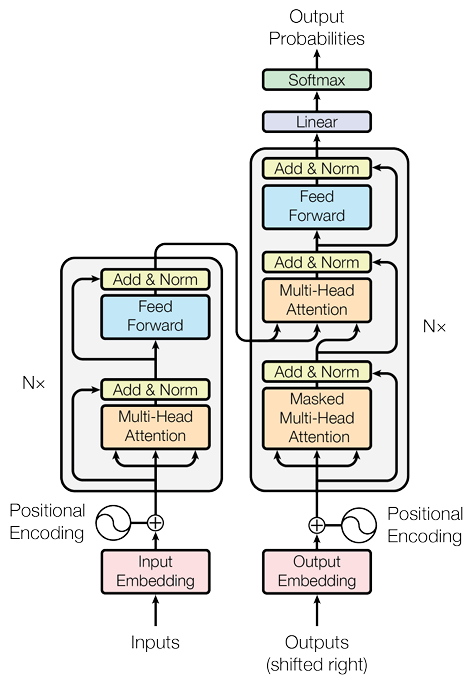
\includegraphics[width=0.5\linewidth]{./images/Transformers architechture from attention is all u need 2017 .png}
    \caption{Model General Architecture \cite{vaswani2017attention}.}
    \label{fig:Attention}
\end{figure}

\subsection{Encoder and Decoder Stacks}
\subsubsection{Encoder}
The encoder consists of $N = 6$ identical layers.  
Each layer contains two sub-layers:
\begin{itemize}
    \item Multi-head self-attention mechanism
    \item Position-wise fully connected feed-forward network (FFN)
\end{itemize}

Each sub-layer is wrapped with a residual connection followed by layer normalization:
\begin{equation}
\text{LayerNorm}(x + \text{Sublayer}(x))
\end{equation}

All sub-layers and embedding layers produce outputs of dimension $d_{\text{model}} = 512$.

\subsubsection{Decoder}
The decoder also consists of $N = 6$ identical layers.  
Each layer contains three sub-layers:
\begin{itemize}
    \item Masked multi-head self-attention
    \item Encoder-decoder attention
    \item Position-wise feed-forward network
\end{itemize}

\paragraph{Note on Hyperparameter Configuration:} 
It is critical to note that dimensions such as $N=6$, $d_{\text{model}}=512$, and $h=8$ represent the baseline configuration established by Vaswani et al. \cite{vaswani2017attention} for NLP. In modern architectural design, particularly for Spatio-Temporal NIDS, these values are treated as tunable hyperparameters rather than fixed constraints, optimized for network traffic features and other requirements.

\subsection{Scaled Dot-Product Attention}
The attention function operates on queries $Q$, keys $K$, and values $V$:
\begin{equation}
\text{Attention}(Q,K,V) = \text{softmax}\left(\frac{QK^T}{\sqrt{d_k}}\right)V
\end{equation}
Scaling by $\sqrt{d_k}$ prevents large dot products from pushing the softmax into regions with very small gradients.

\subsection{Multi-Head Attention and Positional Encoding}
Instead of performing a single attention function, queries, keys, and values are linearly projected $h$ times:
\begin{equation}
\text{MultiHead}(Q,K,V) = \text{Concat}(\text{head}_1, \dots, \text{head}_h) W^O
\end{equation}
Because the Transformer has no recurrence or convolution, positional information must be added to the embeddings using sinusoidal functions so the model can capture the sequential order of network packets.

\section{Vision Transformers (ViT) as a Stepping Stone}
While standard Transformers excelled at NLP, applying them to multidimensional matrices required the \textbf{Vision Transformer (ViT)} \cite{dosovitskiy2020vit}. ViT challenges the dominance of CNNs by treating 2D matrices as sequences of patches. 

\begin{figure}[H]
    \centering
    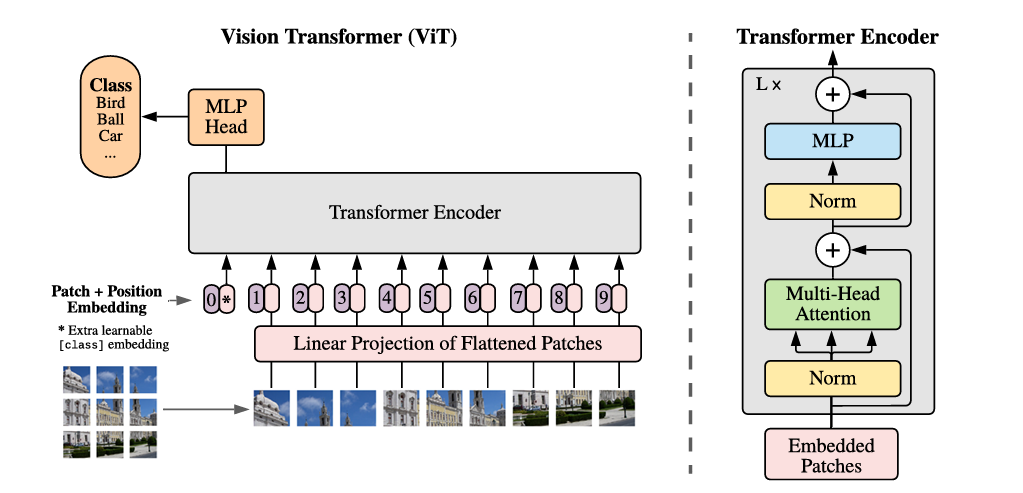
\includegraphics[width=1\linewidth]{./images/vitmodelarchitechrture2020animaheiswort16x16.png}
    \caption{Model overview \cite{dosovitskiy2020vit} .}
    \label{fig:ViT}
\end{figure}

The ViT model divides an input grid into non-overlapping 2D patches, flattening them into a sequence length $N = \frac{H \times W}{P^2}$. Similar to BERT \cite{devlin2019bert}, a \texttt{[class]} token is prepended to serve as the global representation. While ViT proves that self-attention can handle spatial matrices, adapting this strictly to 2D network anomaly detection still fundamentally ignores the temporal dimension of evolving packet flows. This limitation necessitates the evolution into Spatio-Temporal architectures.

\section{Self-Supervised Learning and Masked Autoencoders}
\label{sec:ssl}
To solve the dependency on labeled zero-day attack data, we turn to Self-Supervised Learning (SSL). SSL formulates a "pretext task" where the supervision signal is generated automatically from unlabeled data \cite{balestriero2023cookbook}.


The success of Self-Supervised Learning (SSL) in Natural Language Processing was largely driven by Masked Language Modeling (MLM), popularized by architectures like BERT \cite{devlin2019bert}. Similarly, Computer Vision experienced a paradigm shift through Masked Image Modeling (MIM) via Masked Autoencoders (MAE) \cite{he2022masked}

The Masked Autoencoder is a highly efficient architecture for generative SSL. It relies on an asymmetric design:
\begin{itemize}
    \item \textbf{Asymmetric Encoder:} The input sequence is heavily masked (around $70\%$). The encoder processes only the small subset of visible tokens, significantly reducing computational overhead.
    \item \textbf{Lightweight Decoder:} The decoder reconstructs the original signal from the latent representations and learned ``mask tokens.''
\end{itemize}

The optimization objective minimizes the Mean Squared Error (MSE) strictly on the masked tokens:
\begin{equation}
\mathcal{L}_{MSE} = \frac{1}{|M|} \sum_{i \in M} \| x_i - \hat{x}_i \|^2
\label{eq:mae_loss} 
\end{equation}
This generative self-supervision is highly effective for NIDS. Because the model is trained exclusively on normal traffic, any anomalous packet sequence will violate learned correlations, resulting in a higher MSE anomaly score.


\section{Masked Flow Modeling (MFM)}
\label{sec:mfm}

MFM was designed to address the inefficiencies and redundancies in spatial-domain masking and to leverage the unique properties of the frequency domain for more effective representation learning \cite{xie2023mfm}.

 MFM masks and predicts in the frequency domain, where different frequency components capture different aspects of the data (e.g, low frequencies for global structure, high frequencies for fine details). This approach reduces redundancy and creates a more meaningful self-supervised task.

\subsection{The Mechanics of MFM}
In Masked frequency Modeling, a continuous network flow (comprising a sequence of packets, temporal features, or spatio-temporal tubelets) is divided into discrete tokens. During the pre-training phase. 

The architecture's encoder processes exclusively the unmasked (visible) tokens, extracting deep contextual representations. Subsequently, the decoder attempts to predict or reconstruct the original, uncorrupted values of the masked tokens based purely on the bidirectional spatial and temporal context of the visible tokens \cite{xie2023mfm}.

Mathematically, given a flow sequence $X = \{x_1, x_2, \dots, x_T\}$, a subset of indices $M$ is chosen for masking. The objective is to minimize the reconstruction loss $\mathcal{L}_{\text{MFM}}$ strictly over the masked tokens:
\begin{equation}
\mathcal{L}_{\text{MFM}} = \sum_{i \in M} \text{Loss}(x_i, \hat{x}_i)
\end{equation}
where $\hat{x}_i$ is the predicted token reconstructed by the decoder. For continuous network features, this loss function is typically expressed as the Mean Squared Error (MSE).

\paragraph{MFM as an Anomaly Detection Trigger}
MFM is well suited for Network Intrusion Detection Systems (NIDS). Traditional supervised learning relies heavily on labeled attack data, creating inherent vulnerabilities to zero-day exploits. By employing MFM as a pretext task, the Transformer model learns the intrinsic syntax, structural dependencies, and temporal dynamics of purely \textit{benign} network traffic without requiring human annotation.

When deployed for anomaly detection, the MFM framework calculates the reconstruction error of incoming, real-time traffic. Legitimate flows will closely match the learned syntax, yielding a low reconstruction error. Conversely, malicious traffic—such as Advanced Persistent Threats (APTs) or zero-day malware—inherently violates the learned temporal and spatial correlations of benign traffic. The decoder will fail to reconstruct these anomalous sequences, resulting in a severe spike in the Mean Squared Error. This reconstruction failure serves as a highly accurate, dynamic intrusion alert.


\section{Spatio-Temporal Transformers for Network Topologies}


A Spatio-Temporal Transformer, is a deep learning architecture designed to model data that evolves across both space and time. Its main objective is to learn relationships between entities observed at different positions or feature locations and at different time steps. Unlike classical recurrent models, which process sequences step by step, transformers rely on self-attention to capture short-range and long-range dependencies in parallel. This makes them especially suitable for complex multivariate sequences in which relevant interactions may occur across distant times or across multiple components of the input.

In a general setting, the input can be represented as a sequence of structured observations:
$$
X = \{x_1, x_2, \dots, x_T\}
$$
where each $x_t$ is not simply a scalar but a multidimensional observation describing the system at time $t$. In many applications, each $x_t$ may itself contain several spatial components, feature channels, patches, nodes, sensors, or tokens. The purpose of the STT is to jointly model:
$$
\text{spatial relationships} \quad+\quad \text{temporal relationships}
$$


Standard 2D image models (like ViT) ignore temporal relations, making them unsuitable for continuous sequence predictions. Conversely, sequence models ignore topological structure. By extending into 3D architectures, we represent collected network data as a 3D volume (cube or cuboid), where spatial network features form the 2D grid, and time serves as the third dimension.

\begin{figure}[H]
    \centering
    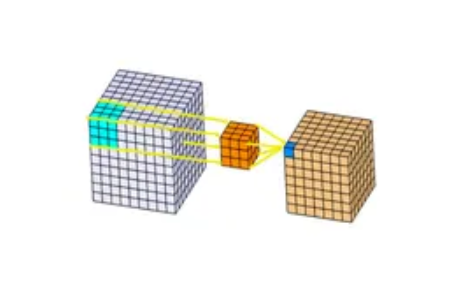
\includegraphics[width=0.5\linewidth]{cube time space .png}
    \caption{Representation of the network data in 3D}
    \label{fig:3D}
\end{figure}


\textbf{However} the term \textbf{spatial}  does not always mean physical 2D or 3D space. More generally, it refers to the structure internal to each observation at a given time step. Depending on the application:
\begin{itemize}
\item image patches in computer vision
\item body joints in human motion modeling
-\item sensors in IoT data
\item graph nodes in traffic networks
\end{itemize}

Thus, the spatial dimension represents how components within the same time step relate to one another.


The \textbf{temporal} dimension represents how the observations evolve over time. It captures:
\begin{itemize}
    \item sequential order
    \item short-term transitions
    \item long-term dependencies
    \item recurring patterns
    \item abrupt changes
    \item trends and periodicity
  
\end{itemize}

In other words, temporal modeling analyses how the current state depend on past and future states.

\subsection{STT Concept}
The central concept of an STT is to first encode each input element into a latent representation and then use self-attention to allow each token to interact with all others. This lets the model learn which parts of the spatio-temporal sequence are relevant for reconstructing, predicting, or classifying the data.

If the input sequence is tokenized into embeddings:
$$
Z = \{z_1, z_2, \dots, z_N\}, \quad z_i \in \mathbb{R}^{d}
$$
then self-attention computes contextualized representations by comparing tokens through query, key, and value projections:
$$
Q = ZW_Q,\quad K = ZW_K,\quad V = ZW_V
$$
and then:
$$
\text{Attention}(Q,K,V) = \text{softmax}\left(\frac{QK^\top}{\sqrt{d_k}}\right)V
$$

This operation allows each token to attend to all other tokens, thereby learning both local and global relationships.


\section{Spatio-Temporal Transformer (STT) Foundations}

\subsection{Generalized Architecture}
A robust STT architecture functions as a multi-stage pipeline designed to map raw, time-varying signals into a structured latent space. The generalized framework consists of five primary modules:

\begin{enumerate}
    \item \textbf{Input Tokenization:} The raw input is decomposed into discrete tokens. Depending on the domain, a token may represent a spatial patch (Computer Vision), a sensor vector (IoT), or a single packet's feature vector (Cybersecurity).
    
    \item \textbf{Latent Projection (Embedding Layer):} Each token $x_i$ is projected into a high-dimensional latent space $d_{model}$ via a learnable linear transformation:
    \begin{equation}
        e_i = \mathbf{W}_{emb} x_i + \mathbf{b}_{emb}
    \end{equation}

In other words to process this 3D volume, the model extracts ``tubelets'' small 3D blocks of data spanning across both the spatial network features and temporal time-windows. 

\begin{figure}[H]
    \centering
    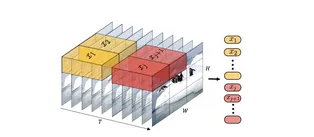
\includegraphics[width=0.5\linewidth]{images/tuplet embengin for stt.png}
    \caption{Visualisation of the tubelet embedding}
    \label{fig:Embedding}
\end{figure}

The tubelet is flattened into a vector representation $z \in \mathbb{R}^{D}$, making volumetric spatio-temporal information strictly compatible with the Transformer architecture.


    
    \item \textbf{Encoding Order (Positional \& Temporal):} As Transformers are permutation-invariant, we inject structural information by adding positional encodings $p_i$:
    \begin{equation}
        h_i = e_i + p_i
    \end{equation}
    This ensures the model distinguishes between "Feature A at Time 1" and "Feature A at Time 10."
    
    \item \textbf{Transformer Encoder Blocks:} A stack of $L$ layers, each containing \textit{Multi-Head Self-Attention (MHSA)} and \textit{Feed-Forward Networks (FFN)}, processes the tokens in parallel to capture global dependencies.
    
    \item \textbf{Task-Specific Head:} The final hidden states are passed to a specialized head for objectives such as \textbf{Anomaly Detection}, \textbf{Traffic Forecasting}, or \textbf{Masked Reconstruction}.
\end{enumerate}

[Image of Spatio-Temporal Transformer (STT) architecture diagram]

\subsection{Spatial and Temporal Attention Strategies}
The efficiency of an STT depends heavily on how it reconciles the two dimensions of data:
\begin{itemize}
    \item \textbf{Joint Attention:} A single self-attention mechanism processes all spatio-temporal tokens simultaneously. While exhaustive, it suffers from $O((T \times S)^2)$ complexity.
    \item \textbf{Factorized Attention:} The model alternates between spatial attention (within a time step) and temporal attention (across time steps). This reduces computational overhead while maintaining structural hierarchy \cite{bertasius2021space}.
    \item \textbf{Hierarchical Attention:} Local patterns are learned first and subsequently aggregated into global representations, mimicking the receptive field expansion of CNNs.
\end{itemize}















\subsection{Hyperparameters}
Hyperparameters are external settings that are defined before training begins and control how the model learns . The prefix `hyper-' indicates that these are `top-level' parameters that govern the learning process itself rather than being part of the resulting model.

Key characteristics of hyperparameters:
\begin{itemize}
    \item External settings defined before training that control how the model learns.
    \item Not learned by the model, but chosen manually or through optimization techniques.
    \item External to the model and not part of the final trained model.
    \item Critical for model performance and generalization ability.
\end{itemize}

Examples of hyperparameters:
\begin{itemize}
    \item \textbf{Learning rate:} Controls how fast parameters are updated during training, affecting convergence speed and stability.
    \item \textbf{Number of epochs:} Determines how many times the model sees the full dataset during trainin.
    \item \textbf{Batch size:} Number of samples processed before updating parameters, influencing training efficiency and memory usage .
    \item \textbf{Number of layers/neurons in neural networks:} Architecture decisions that determine model capacity and complexity .
    \item \textbf{Regularization strength (e.g., L1/L2):} Controls overfitting by penalizing large parameter values .
    \item \textbf{Number of trees/depth in Random Forest or Gradient Boosting:} Ensemble specific parameters affecting model complexity and performance .
    \item \textbf{Choice of activation function:} Determines the non-linear transformation applied to neuron outputs. Examples include ReLU, Sigmoid, Tanh, Leaky ReLU, ELU, and Swish .
    \item \textbf{Choice of optimizer:} Determines the algorithm used to update model parameters during training. Examples include SGD, Adam, RMSprop, AdaGrad, and Nadam .
\end{itemize}

The distinction between parameters and hyperparameters is fundamental to machine learning: while parameters define what the model has learned, hyperparameters define how the learning process itself is conducted . Both are essential for developing effective machine learning models, but they serve different purposes and require different approaches for optimization and selection.

\section{Activation Functions and Loss Design}

\subsection{Sigmoid, Softmax, and GELU}
Deep neural networks rely on nonlinear mappings to transform latent representations into decision scores. In binary classification, a scalar logit $z$ is commonly converted into a probability through the sigmoid function:
\begin{equation}
\sigma(z)=\frac{1}{1+e^{-z}}.
\end{equation}
The sigmoid squashes any real-valued score into the interval $[0,1]$, which makes it suitable for binary decisions such as malicious versus benign traffic.

For multi-class classification, the corresponding mapping is the softmax function. Given a vector of logits $z = (z_1,\dots,z_C)$ over $C$ classes, the softmax probability assigned to class $c$ is
\begin{equation}
\operatorname{softmax}(z)_c = \frac{e^{z_c}}{\sum_{k=1}^{C} e^{z_k}}.
\end{equation}
Unlike sigmoid, which treats one score independently, softmax normalizes all class scores jointly and produces a full categorical distribution whose entries sum to one.

Inside Transformer feed-forward and decoder blocks, smoother hidden activations are often preferred. One widely used choice is the Gaussian Error Linear Unit (GELU), defined as
\begin{equation}
\operatorname{GELU}(x)=x\,\Phi(x),
\end{equation}
where $\Phi(x)$ is the cumulative distribution function of the standard Gaussian. GELU can be interpreted as a smooth gating mechanism: small or uncertain activations are softly attenuated, while larger informative activations pass through more strongly. This makes GELU especially popular in modern Transformer architectures.

\subsection{Robust Regression and Multitask Objectives}
Not all learning objectives in deep models are pure classification losses. In self-supervised reconstruction, the model must predict continuous values, which turns the problem into a regression task. A common baseline is the Mean Squared Error (MSE), but MSE can be overly sensitive to large outliers. A more robust alternative is the SmoothL1 loss, also known as a Huber-like loss, which behaves quadratically for small errors and linearly for large ones:
\begin{equation}
\ell_{\mathrm{SmoothL1}}(a,b)=
\begin{cases}
\frac{1}{2}(a-b)^2, & |a-b|<1, \\
|a-b|-\frac{1}{2}, & |a-b|\ge 1.
\end{cases}
\end{equation}
Here, $a$ denotes the prediction and $b$ the target value. Because the penalty becomes linear beyond the transition point, SmoothL1 is less dominated by a small number of extreme residuals than MSE.

In multitask learning, several objectives are optimized simultaneously. The total loss is typically written as a weighted combination,
\begin{equation}
\mathcal{L}=\sum_{m=1}^{M} \lambda_m\mathcal{L}_m,
\end{equation}
where $\mathcal{L}_m$ is the loss associated with task $m$ and $\lambda_m$ controls its contribution to the total objective. This design is useful when one shared backbone must support binary detection, family classification, forecasting, anomaly scoring, and auxiliary reconstruction at the same time.

\section{Model Evaluation Metrics}

\subsection{Accuracy, Precision, Recall, and F1-Score}
The evaluation of machine learning models requires multiple metrics to capture different aspects of performance. The most fundamental metrics are derived from the confusion matrix, which contains True Positives (TP), True Negatives (TN), False Positives (FP), and False Negatives (FN) .

\begin{itemize}
    \item \textbf{Accuracy} is the ratio between correctly classified samples and the total number of samples, calculated as:
    \begin{equation}
        \text{Accuracy} = \frac{TP + TN}{TP + TN + FP + FN} \in [0,1]
        \label{eq:accuracy}
    \end{equation}
    However, accuracy can be misleading in cases of class imbalance.

    \item \textbf{Recall}, also known as sensitivity or True Positive Rate (TPR), denotes the rate of positive samples correctly classified:
    \begin{equation}
        \text{Recall} = \frac{TP}{TP + FN} \in [0,1]
        \label{eq:recall}
    \end{equation}
    This metric is particularly important in medical applications (and cybersecurity) where missing positive instances should be minimized.

    \item \textbf{Precision} represents the proportion of correctly classified positive samples among all samples assigned to the positive class:
    \begin{equation}
        \text{Precision} = \frac{TP}{TP + FP} \in [0,1]
        \label{eq:precision}
    \end{equation}
    High precision indicates that the model makes few false positive errors.

    \item \textbf{The F1-score} is the harmonic mean of precision and recall, providing a balanced measure:
    \begin{equation}
        F1 = 2 \cdot \frac{\text{Precision} \cdot \text{Recall}}{\text{Precision} + \text{Recall}} \in [0,1]
        \label{eq:f1_score}
    \end{equation}
    This metric is particularly useful when there is an uneven class distribution.
\end{itemize}

\subsubsection{Confusion Matrix}
A confusion matrix is defined as a table used to visualize the performance of a classifier, with rows and columns representing each class. For binary classification, it takes the form of a $2 \times 2$ matrix containing the counts of TP, TN, FP, and FN observations. The confusion matrix provides a comprehensive view of model performance, showing not only correct classifications but also the types of errors being made. This detailed breakdown is essential for understanding model behavior and identifying specific areas for improvement .

\subsubsection{Receiver Operating Characteristic (ROC) Curve and Area Under Curve (AUC)}
The Receiver Operating Characteristic (ROC) curve is a graphical plot that illustrates the diagnostic ability of a binary classifier as its discrimination threshold is varied. The curve plots the true positive rate (sensitivity) against the false positive rate ($1 - \text{specificity}$) at various threshold settings. The Area Under the ROC Curve (AUC) provides a single scalar value that summarizes the performance across all possible thresholds .

AUC exhibits several desirable properties compared to overall accuracy: increased sensitivity in Analysis of Variance (ANOVA) tests, a standard error that decreases as both AUC and the number of test samples increase, decision threshold independence, and invariance to a priori class probabilities . For these reasons, AUC is often preferred over overall accuracy for single-number evaluation of machine learning algorithms.

\subsubsection{Precision--Recall Curve}
Precision-Recall (PR) curves are particularly useful for evaluating classifiers on highly skewed datasets. Unlike ROC curves, PR curves focus on the performance of the positive class, making them more informative when the negative class dominates the dataset. The curve plots precision against recall at various threshold settings, providing a clear picture of the trade-off between these two metrics .

A deep connection exists between ROC space and PR space, such that a curve dominates in ROC space if and only if it dominates in PR space  However, there are important differences: in PR space, it is incorrect to linearly interpolate between points, and algorithms that optimize the area under the ROC curve are not guaranteed to optimize the area under the PR curve. This makes PR curves essential for evaluating models on imbalanced datasets common in intrusion detection tasks.

\subsubsection{Open-Set and Out-of-Distribution Evaluation}
Classical closed-set classification assumes that every test sample belongs to one of the classes observed during training. In cybersecurity, this assumption is often unrealistic because genuinely new attack families can appear after deployment. Open-set recognition relaxes the closed-set assumption and requires the model not only to classify known classes, but also to reject samples that do not match the learned label vocabulary with sufficient confidence.

This distinction is especially important for Network Intrusion Detection Systems. A model can achieve strong performance on in-distribution traffic while still failing on genuinely novel attacks. For this reason, modern IDS evaluation often includes a stricter out-of-distribution (OOD) protocol in which one or more attack families are held out during training and reserved for testing. The purpose is not merely to measure accuracy on familiar classes, but to assess whether the system can remain reliable when the attack distribution shifts beyond the supervised training regime.

\subsubsection{Threshold Selection and Score Calibration}
Many IDS models produce continuous scores rather than hard labels. A deployed decision is obtained by comparing a score to a threshold $\tau$. This leads to an important distinction between threshold-free metrics and thresholded metrics. Measures such as ROC-AUC or PR-AUC quantify ranking quality across all possible thresholds, whereas operational precision, recall, and F1-score depend directly on the chosen operating point.

In practice, thresholds should be selected on a validation split and then frozen before test evaluation. This prevents optimistic bias and makes the reported deployment scenario more realistic. For anomaly scores, an additional calibration step is often used to convert a raw score $s$ into an interpretable confidence value relative to a reference validation distribution $V$:
\begin{equation}
\hat{p}(s)=\frac{1}{|V|}\sum_{u\in V} \mathbf{1}[u \le s],
\end{equation}
where $\mathbf{1}[\cdot]$ is the indicator function. This percentile-based view measures how extreme the observed score is compared with reference traffic. It also explains why ranking metrics can remain high while thresholded recall collapses under distribution shift: if the score ordering is still informative but the validation-selected threshold no longer matches the new score distribution, the deployed decision rule may fail even though the model still separates samples reasonably well.

\subsubsection{Training and Validation Loss Curves}
Training and validation loss curves are fundamental tools for monitoring the learning process of neural networks and detecting issues such as overfitting and underfitting. During training, the optimization algorithm tries to minimize the cost function of the network, and the loss curves show how this metric changes over epochs .

Analysis of these curves allows for early detection of training issues, enabling timely interventions such as early stopping, learning rate adjustment, or model architecture modifications to improve performance and prevent wasted computational resources.








\part{State of the Art}
\chapter{sota}
\section{Introduction}
This chapter provides a comprehensive review of recent literature addressing Network Intrusion Detection Systems (NIDS) utilizing advanced machine learning techniques. The purpose is to present the main datasets and methodologies that have been proposed. 

To track the evolution of the field and highlight the gaps that necessitate our proposed architecture, the state-of-the-art papers are grouped thematically by their core approach to processing network data. 

We transition from models that attempt to map network data into 2D visual representations, to those treating flows as NLP-style sequences, moving to cutting-edge models exploring Graph and Spatio-Temporal topologies, and finally the detection of zero-day attacks.

\section{Datasets}

 To accurately simulate network environments, exercise  testing  and  integrate proposed solutions, the cybersecurity community relies on baseline traffic captures. 
 In this section, we present an overview of the most prominent benchmark datasets utilized in the state-of-the-art literature, highlighting their specific network topologies.

% --- Proceed to describe the specific datasets --

\subsubsection{KDD-99:}

  The 1999 KDD intrusion detection contest uses a standard set of data \cite{kddcup99} which includes a wide variety of intrusions simulated in a military network environment.The purpose is to audit  and evaluate research in intrusion detection ,
  Labs set up an environment to acquire nine weeks of raw TCP dump data for a local-area network (LAN) simulating a typical U.S. Air Force LAN. .

The raw training data was about four gigabytes of compressed binary TCP dump data from seven weeks of network traffic.  This was processed into about five million connection records.  Similarly, the two weeks of test data yielded around two million connection records.


Attacks fall into four main categories

\begin{itemize}
    \item \textbf{DOS (Denial of Service):} Attempts to shut down or overload a network (e.g., SYN flood).
    \item \textbf{R2L (Remote to Local):} Unauthorized remote access attempts (e.g., password guessing).
    \item \textbf{U2R (User to Root):} Unauthorized escalation of local privileges (e.g., buffer overflows).
    \item \textbf{Probing:} Surveillance and scanning to find vulnerabilities (e.g., port scanning).
\end{itemize}


\subsubsection{NSL-KDD:}
NSL-KDD \cite{kdd2009datset} is a dataset suggested to solve some of the inherent problems of the KDD'99 dataset

\subsubsection{CIC-IDS2017:}
CIC-IDS2017 \cite{CICIDS2017}, was developed by the Canadian Institute for Cybersecurity (CIC), represents a critical milestone in NIDS evaluation. It was specifically engineered to address the severe architectural shortcomings and lack of modern threat representation found in legacy benchmarks like KDD Cup 99 and NSL-KDD \cite{sharafaldin2018toward}. 

Unlike older, purely synthetic datasets, \textbf{CIC-IDS2017} captures highly realistic background traffic which extracts and simulates the abstract behavior of genuine human interactions (e.g., HTTP, HTTPS, FTP, SSH, and email protocols). The dataset encompasses five days of dense network activity, featuring a comprehensive taxonomy of modern attack vectors categorized as follows:
\begin{itemize}
    \item \textit{DDoS} and \textit{Dos} 
    \item \textit{Web Attacks} and \textit{Brute Force}
    \item \textit{Infiltration} and \textit{PortScans} 
    \item \textit{Botnets}
\end{itemize}


\subsubsection{CIC-IDS2018:}

The CSE-CIC-IDS2018 \cite{cic2018dataset} dataset is a large-scale, dynamically generated benchmark. Created as a collaborative project between the Communications Security Establishment (CSE) and the Canadian Institute for Cybersecurity (CIC) on the AWS cloud computing platform, this dataset addresses the critical limitations of older static benchmarks by providing realistic, up-to-date traffic compositions. It is  a direct evolution of the CIC-IDS2017 dataset.
 
To synthesize a highly realistic network environment, the dataset utilizes a profile-based generation methodology. The key characteristics of this approach include:

\begin{itemize}
    \item \textbf{B-Profiles (Benign Profiles):} These encapsulate the naturalistic behavior of human users by leveraging machine learning and statistical analysis techniques to simulate standard protocols such as HTTP, HTTPS, FTP, SSH, and email.
    
    \item \textbf{M-Profiles (Malicious Profiles):} These introduce seven distinct, modern attack scenarios into the network, specifically: Brute-force, Heartbleed, Botnets (Zeus and Ares), DoS, DDoS, Web attacks, and internal network infiltration.
    
    \item \textbf{Diverse Topology:} The dataset simulates a complex organizational infrastructure comprising 5 departments, 30 servers, and 420 victim machines running various Windows and Linux operating systems. This internal network is targeted by an external attacking infrastructure of 50 machines.
    
    \item \textbf{Comprehensive Data Sources:} For advanced cybersecurity and machine learning research, the dataset is exceptionally thorough. It provides raw network traffic captures (PCAPs) and system event logs (from both Windows and Ubuntu environments) for researchers who wish to build custom feature extractors.
\end{itemize}


\subsubsection{UNSW-NB15:}


The UNSW-NB15 dataset is a comprehensive network intrusion detection benchmark generated in the Cyber Range Lab of UNSW Canberra \cite{UNSW-NB15dataset}. Created to provide a highly realistic evaluation environment, the dataset utilizes the \textit{IXIA PerfectStorm} emulation tool to synthesize a hybrid manifold of real, modern, normal network activities alongside contemporary synthetic attack behaviors.

The underlying composition of the dataset is organized as follows:

\begin{itemize}
    \item \textbf{Traffic Volume and Ingestion:} The raw network captures consist of approximately $100\text{~GB}$ of raw traffic captured via the \texttt{tcpdump} utility and archived in native PCAP format. 
    \item \textbf{Attack Taxonomy:} The malicious traffic profiles encompass nine distinct structural categories of cyber-attacks:
    \begin{itemize}
        \item \textit{Fuzzers} and \textit{Analysis}
        \item \textit{Backdoors} and \textit{Exploits}
        \item \textit{DoS} and \textit{Worms}
        \item \textit{Generic}, \textit{Reconnaissance}, and \textit{Shellcode}
    \end{itemize}
    \item \textbf{Feature Extraction Pipeline:} To facilitate advanced machine learning applications, the dataset creators deployed a pipeline leveraging \texttt{Argus}, \texttt{Bro-IDS} (Zeek), and twelve specialized custom heuristic algorithms to extract $49$ distinct multivariate features embedded with corresponding ground-truth class labels.
\end{itemize}

In its entirety, the complete dataset contains $2,540,044$ connection records structurally distributed across four tabular CSV files, which are accompanied by a dedicated ground-truth table and an event list. 

To guarantee reproducibility and uniform baseline testing across comparative research studies, a standardized subset has been formally partitioned into two non-overlapping sets: a dedicated training set containing $175,341$ records and a test set containing $82,332$ records. Both partitions maintain a complex, mathematically balanced mixture of benign baseline communication profiles and active threat vectors.





% --- CATEGORY 1: VISUAL ---
\section{Visual Representation and Image-Based Models}
A significant branch of recent research attempts to bypass the limitations of tabular data by mathematically transforming network packets and flows into 2D. This allows the utilization of mature Computer Vision architectures (like CNNs and ViTs) for anomaly detection.

\subsection{Xu \& al., "Falcon" 2021}
Introduces \cite{xu2021falcon}, an Android malware detection framework that treats network traffic classification as a 2D image sequence classification problem.The framework was trained and evaluated using the \textbf{Android Malware CICMal2017 dataset}, which includes 426 malware and 1700 benign samples. From 2,126 raw PCAP files, the authors extracted over 3,255,391 total network flows.

\subsubsection{Architecture and Solution}
\begin{itemize}
    \item \textbf{Network Flows to Images:} Packets are converted into 2D grayscale images by trimming or padding flows to ensure a uniform 784-byte size.
    \item \textbf{Continuous Traffic Processing:} A pre-trained 8-layer CNN extracts vectors, which are then passed through a bi-directional LSTM network to capture temporal sequential relationships between the 2D packet images.
\end{itemize}

\subsubsection{Experimental Results}
\begin{itemize}
    \item Evaluated on the used Dataset achieved an accuracy of 97.16\% in binary classification and 84.70\% in multi-class categorization. The model was tested against various classifiers, including AdaBoost, GradientBoost, MLP, and DecisionTree. The \textbf{Random Forest} classifier achieved the best performance with an accuracy of 97.16, precision of, 97.13, recall of 97.16, and an F1-score of 97.09.
\end{itemize}

\subsection{L. Mohammadpour \& al., "CNN-Based IDS Survey" 2022}
This survey \cite{mohammadpour2022survey} provides a comprehensive study on a CNN-based IDS, categorizing it into four main approaches: single CNN models, hybrid CNN-RNN architectures (combining CNNs with LSTMs or GRUs for spatial-temporal feature extraction), hybrid CNNs with deep learning models (like autoencoders), and hybrid CNNs paired with machine learning algorithms.It also analyzes architectures, hyperparameter settings, and input dimension types (1D vs. 2D).

\subsubsection{Architecture and Solution}
\begin{itemize}
    \item Highlights preprocessing methods used to convert tabular network packets into 2D formats (grayscale matrices) to extract hierarchical correlations without manual feature engineering.
\end{itemize}

\subsubsection{Experimental Results}
\begin{itemize}
    \item Reviews KDD Cup99, NSL-KDD, UNSW-NB15, and CIC-IDS2017. Confirms that hybrid CNN models (e.g., CNN-LSTM) consistently outperform single CNNs by capturing temporal sequences alongside spatial properties. 
\end{itemize}

\subsection{Kim \& al., "Multiple Image Transformers" 2023}
\cite{kim2023deep} introduces an optimized method for converting tabular NIDS datasets into 2D visual representations utilizing multiple image transformers, integrating dimensionality reduction to construct RGB images.

\subsubsection{Architecture and Solution}
\begin{itemize}
    \item \textbf{RGB Image Synthesis:} Employs algorithms (t-SNE, UMAP, PCA) to map numerical features into 2D spatial matrices. The top three are mapped to Red, Green, and Blue channels to synthesize a multi-dimensional RGB image.
    \item \textbf{Dual CNN Classifier:} Utilizes a four-layer dual CNN with parallel convolutional filters to process the generated RGB images.
\end{itemize}

\subsubsection{Experimental Results}
\begin{itemize}
    \item This survey \ proposed multiple-transformer ensemble using 3-channel color images achieved superior performance with an \textbf{Accuracy} of \textbf{95.60} and an \textbf{F1-Score} of \textbf{93.86} on the ISCXIDS2012 dataset. On the CSE-CIC-IDS2018 dataset, the method achieved an \textbf{Accuracy} of \textbf{95.50} and an \textbf{F1-Score} of \textbf{92.52} 
\end{itemize}

\subsection{He \& al., "DE-VIT" 2024}
This study \cite{he2024network} introduces a Deformable Vision Transformer (DE-VIT) to address network intrusion detection by transforming data into image formats. It leverages deformable attention mechanisms to capture global and local features while minimizing computational costs.

\subsubsection{Architecture and Solution}
\begin{figure}[H]
    \centering
    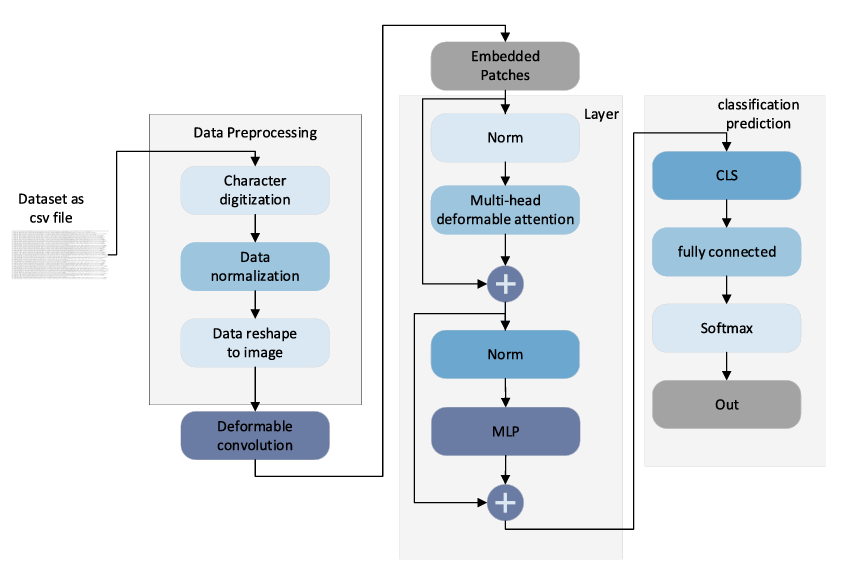
\includegraphics[width=0.7\linewidth]{./images/SOTA2024VIT-IDS.png}
    \caption{Model process \cite{he2024network} }
\end{figure}
\begin{itemize}
    \item \textbf{Data Transformation:} Preprocesses traffic into 64 features and reshapes them into an $8\times8$ image matrix. It applies deformable convolutions with a sliding window to extract image features.
    \item \textbf{Deformable Attention:} Instead of dense self-attention, the model calculates relationships only with surrounding features, reducing overhead.
    \item \textbf{L-Focal Loss:} Implemented to address highly imbalanced datasets.
\end{itemize}

\subsubsection{Experimental Results}
\begin{itemize}
    \item Achieved an \textbf{Accuracy} of 99.5\% on CIC-IDS2017 \cite{canadian2017cicids} and 97.25\% on UNSW-NB15\cite{canadian2017cicids} and produced an exceptional Area Under the Curve \textbf{(AUC)} of 0.995 in binary configurations, significantly outperforming CNN and LSTM baselines. 
\end{itemize}

\subsection{Abed \& al., "A modified CNN-IDS model" 2024}
This study \cite{abed2024modified} addresses supersized data spaces by implementing feature selection techniques prior to image-based CNN classification.

\subsubsection{Architecture and Solution}
\begin{itemize}
    \item \textbf{Dimensionality Reduction:} Employs PCA and Singular Value Decomposition (SVD) to mathematically transform the feature space and discard irrelevant noise.
    \item \textbf{Hybrid Classification:} Evaluates the transformed space using Ridge Regression, Stochastic Gradient Descent, and CNNs to execute threat detection.
\end{itemize}

\subsubsection{Experimental Results}
\begin{itemize}
    \item The study achieved a successful implementation with a \textbf {Precision} around 86.93 to 88.52  precision for UNSW-NB15, and about 93.81 to 99.67 for the WSN‑DS dataset.  
\end{itemize}

\subsection{Xiao Liu \& al., "Mean Masked Autoencoder with Flow-Mixing for Encrypted Traffic Classification" 2026}
Recently, the application of Masked Autoencoders (MAE) for encrypted traffic classification has highlighted the limitations of standard random masking, which is ill-suited for the high semantic density of network packets. To overcome this constraint, Liu et al. (2026) proposed the Mean Masked Autoencoder (MMAE) \cite{liu2026mean}, an architecture leveraging a teacher-student self-distillation paradigm coupled with a Flow-Mixing strategy. This approach replaces conventional masking by injecting cross-flow interference, thereby compelling the model to discriminate features within highly noisy environments. 

While this method improves model robustness, it remains restricted to a strictly spatial modeling of the traffic. In contrast to this flow-mixing approach, our architecture resolves temporal feature extraction through direct modeling in the spectral domain. By introducing Masked Frequency Modeling (MFM) via Fast Fourier Transform (FFT), our foundation model captures the intrinsic spatio-temporal dynamics of an isolated flow, thus bypassing the computational complexity associated with asymmetric flow pairing.


% --- CATEGORY 2: SEQUENTIAL NLP ---
\section{Sequential Flow and NLP-Adapted Transformers}
While visual models successfully mapped spatial correlations, they often struggle with long-term temporal dependencies. Consequently, another major research branch treats network flows identically to sentences in Natural Language Processing (NLP), applying standard sequence-based Transformers.

\subsection{Athul K \& Anita John., "A Deep Learning based Intrusion Detection System using Transformers" 2022}
This study \cite{k2022deep} focuses on minimizing computational complexity by ranking and selecting important security features using NLP models before classification. 

\subsubsection{Architecture and Solution}
\begin{figure}[H]
    \centering
    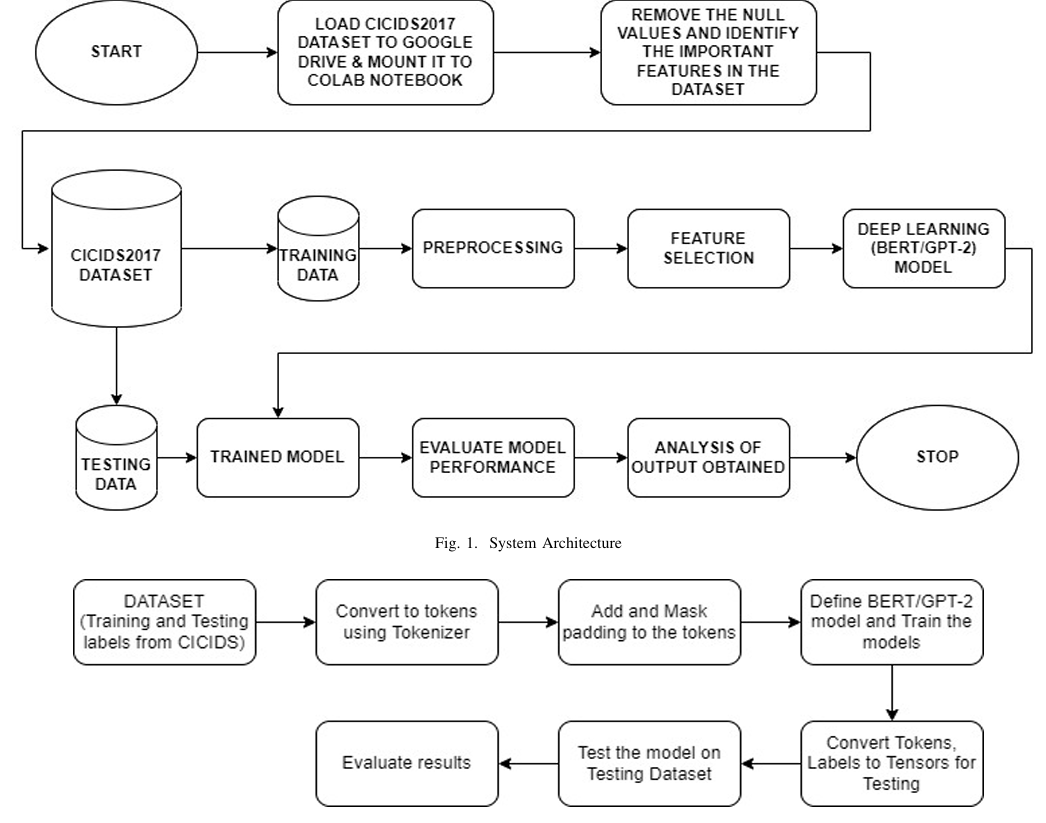
\includegraphics[width=0.8\linewidth]{./images/SOTA-Trans-dl-2022.png}
    \caption{System Design \cite{k2022deep} }
\end{figure}
\begin{itemize}
    \item \textbf{Feature Selection Classification:} The dataset is preprocessed to identify and utilize only the 30 most important features to reduce computational complexity and overhead.
    \item \textbf{Data Transformation Classification:} The framework converts the intrusion and normal records into strings of text sequences. These sequences are then tokenized and parsed into chunks of length six.
    \item \textbf{Padding and Masking:} The tokens are appended with padding and masked, which is a necessary step for the transformer architectures to function properly.
    \item \textbf{Classification:} The processed data is fed into the defined BERT and GPT-2 models for binary classification
\end{itemize}

\subsubsection{Experimental Results}
\begin{itemize}
    \item Evaluated on CICIDS2017. Proved that leveraging NLP transformers for feature dimensionality reduction minimizes computational complexity while maintaining high detection rates. 
\end{itemize}

\subsection{Wu \& al., "RTDIS" 2022}
\cite{wu2022rtids} serves as a foundational baseline demonstrating how transformers effectively handle high-dimensional traffic data without losing critical feature representations.

\subsubsection{Architecture and Solution}
\begin{figure}[H]
    \centering
    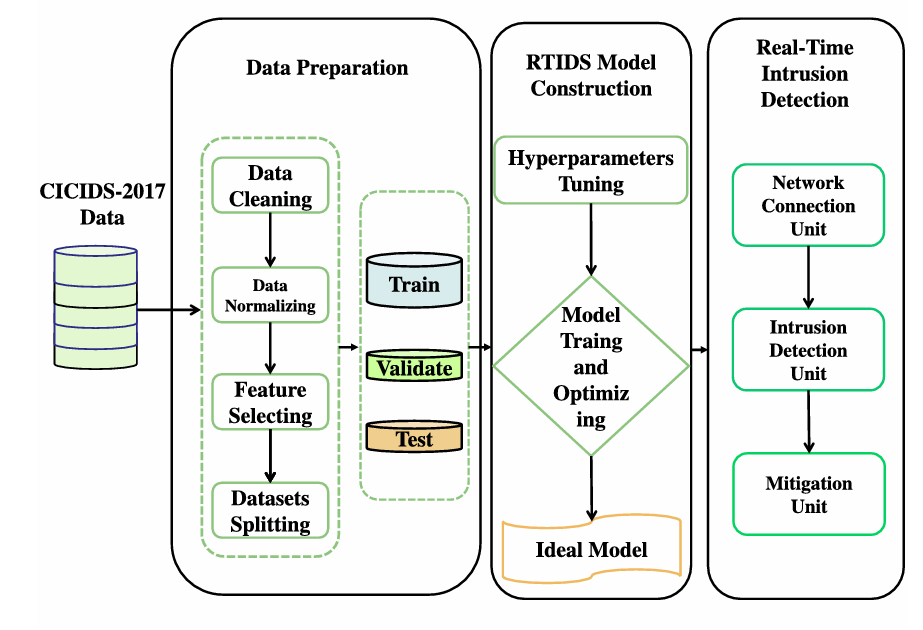
\includegraphics[width=0.8\linewidth]{./images/SOTA2022RTIDS.png}
    \caption{RTDIS model architecture \cite{wu2022rtids} }
\end{figure}
\begin{itemize}
    \item \textbf{Data Balancing:} To combat the severe class imbalance in the datasets and prevent model overfitting, the framework utilizes the Synthetic Minority Oversampling Technique (SMOTE) during preprocessing.
    \item \textbf{Self-Attention Mechanism:} A multi-head self-attention mechanism is applied to learn varying weights of feature representations, bypassing traditional recurrent connections.
    \item \textbf{Masked Decoders for Robustness:} The decoder stack includes an additional masked self-attention sublayer that randomly masks a portion of features.
\end{itemize}

\subsubsection{Experimental Results}
\begin{itemize}
    \item RTIDS achieved an F1-Score of 99.17\% on CICIDS2017 and 98.48\% on CIC-DDoS2019, outperforming baseline models including SVM, RNN, and LSTM. 
\end{itemize}

\subsection{Liu \& al., "Intrusion Detection Model Based on Improved Transformer" 2023}
\cite{liu2023intrusion} addresses three challenges: lengthy training times, inaccurate detection of overlapping classes, and poor multi-class classification by optimizing positional encoding for non-sequential data.

\subsubsection{Architecture and Solution}
\begin{figure}[H]
    \centering
    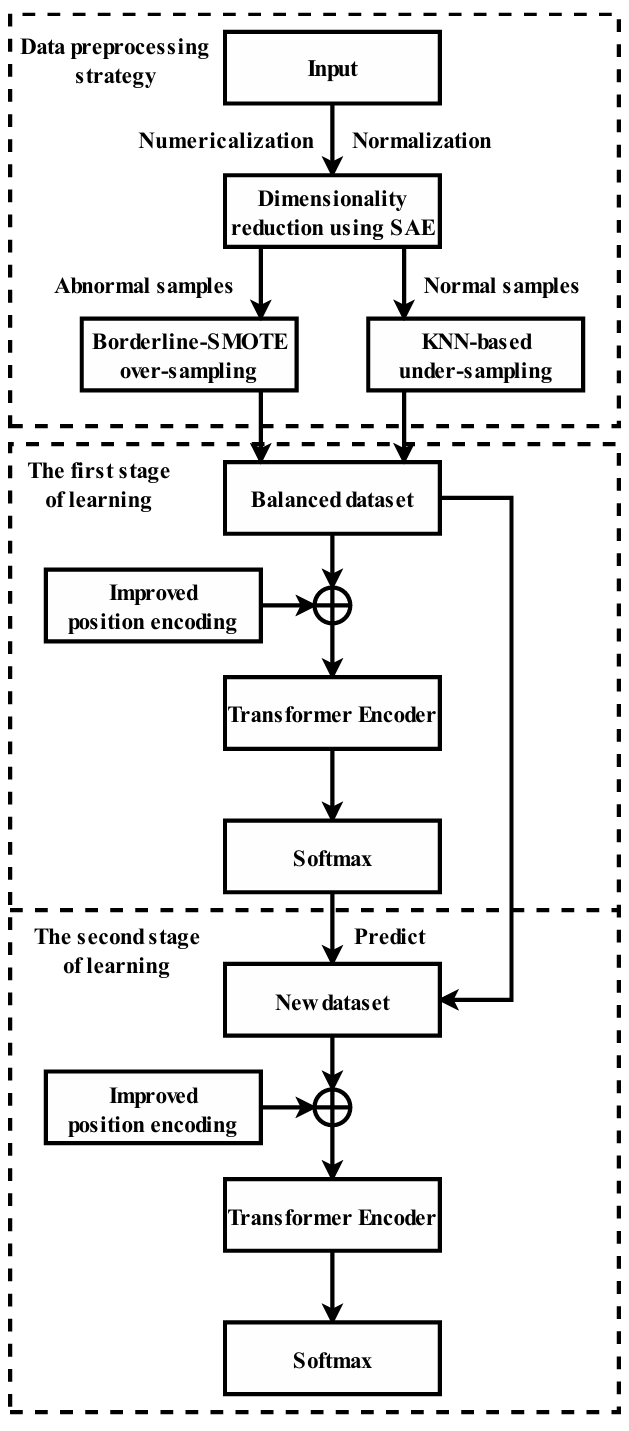
\includegraphics[width=0.45\linewidth]{./images/SOTA2023modelbasedids.png}
    \caption{Improved Transformer-based intrusion detection model \cite{liu2023intrusion} }
\end{figure}
\begin{itemize}
    \item \textbf{Improved Position Encoding:} Standard Transformer encoding is ineffective for independent numerical features. The authors modified the formula to embed the positional index of each feature ($i$) to learn spatial dependencies.
    \item \textbf{Hybrid Sampling \& Two-Stage Learning:} Uses KNN under-sampling and Borderline-SMOTE, followed by a rough binary classification (normal vs. attack) leading into an accurate multi-class prediction.
\end{itemize}

\subsubsection{Experimental Results}
\begin{itemize}
    \item On the NSL-KDD dataset, the model achieved an accuracy of 88.7\% and an F1-score of 88.2\% for binary classification, with a remarkably fast training time of only 8 seconds. For multi-class classification, it recorded an 84.1\% accuracy and an 83.8\%  F1-score. On the UNSW-NB15 dataset, the model achieved 87.5\% accuracy and an 87.3\% F1-score for multi-class classification, completing training in just 19 seconds.
\end{itemize}

\subsection{Manocchio \& al., "FlowTransformer" 2024}
This study \cite{manocchio2024flowtransformer} evaluates various transformer components (input encoding, blocks, heads) for flow-based network traffic. It aims to identify the optimal configurations for NIDS by comparing various transformer architectures, input encodings, and classification heads.

\subsubsection{Architecture and Solution}
\begin{figure}[H]
    \centering
    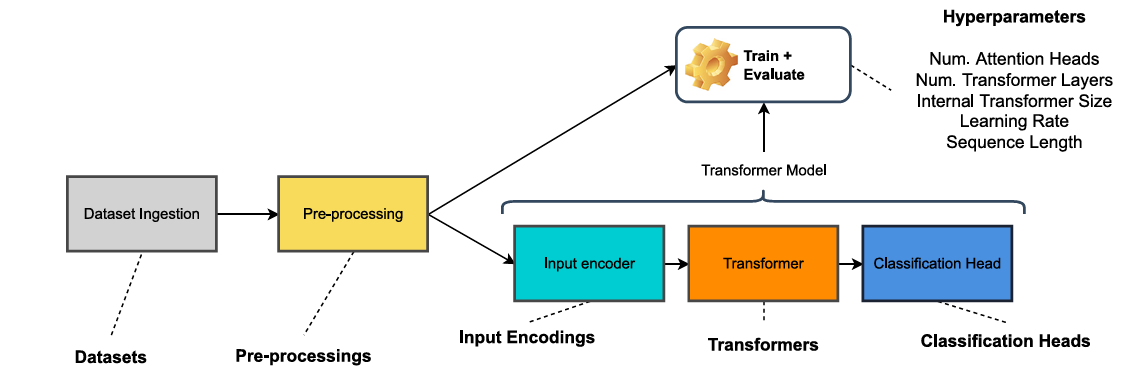
\includegraphics[width=0.95\linewidth]{images/SOTA2024FlowTransformercopie.png}
    \caption{FlowTransformer framework architecture \cite{manocchio2024flowtransformer}. }
\end{figure}
\begin{itemize}
    \item \textbf{Shallow vs. Deep Transformers:} Reveals that shallow transformers (e.g, 2 layers) perform equivalently to deep models (BERT/GPT) in flow-based tasks while offering vastly superior computational throughput.
    \item \textbf{Classification Head:} Proves that the "Last Token" approach significantly outperforms Global Average Pooling for NIDS contexts.
\end{itemize}

\subsubsection{Experimental Results}
\begin{itemize}
    \item It achieved a state-of-the-art F1-Score of 98.00\% on NSL-KDD, 97.05\% on CSE-CIC-IDS2018, and 90.45\% on UNSW-NB15.
\end{itemize}

\subsection{F.Ullah \& al., "IDS-INT" 2024}
In this study \cite{ullah2024ids} the authors created a deep learning-based Intrusion Detection System (IDS) that applies Natural Language Processing (NLP) algorithms—specifically BERT and GPT-2 to detect modern cyber threats. 

\subsubsection{Architecture and Solution}
\begin{itemize}
    \item \textbf{Semantic Tokenization:} Parses PCAP files to extract flow events. It utilizes a BERT large model to compute contextual relationships and extract semantic train features.
    \item \textbf{CNN-LSTM Classifier:} Feeds the BERT-extracted features into a 1D-CNN and LSTM network to capture sequential and temporal dependencies.
\end{itemize}

\subsubsection{Experimental Results}
\begin{itemize}
    \item Tested on UNSW-NB15, CIC-IDS2017, and NSL-KDD. It successfully mitigated majority-class bias and significantly outperformed the baseline methods with an overall 99\% F1-score, and 99.21\% Accuracy.
\end{itemize}

\subsection{Berry \& al., "Explainability of Network Intrusion Detection Using Transformers" 2025}
This study \cite{rajkumardheivanayahi2025explainability} shifts focus from traditional flow-based analysis to a packet-level approach. It addresses open-world recognition by leveraging transformers to generate natural language explanations for unknown network packets.

\subsubsection{Architecture and Solution}

\begin{itemize}
    \item \textbf{Packet Embedding \& Clustering:} Utilizes a fine-tuned \textbf{Bert} model to generate 768-dimensional contextual embeddings for individual packets based on the first 500 payload bytes. It applies k-means clustering to assign network tags.
    \item \textbf{Explainability:} A Falcon-7B decoder-only model is fine-tuned to generate human-readable descriptive sentences explaining the assigned tags and payload contents.
\end{itemize}

\subsubsection{Experimental Results}
\begin{itemize}
    \item Evaluated on CIC-IDS2017 and UNSW-NB15. 
    The fine-tuned BERT model achieved an accuracy of 99.48 and a macro F1-score of 98.46\% on a test set containing over 500,000 packets.
    Also achieved an explainability score of 0.6331 and generated text with 95.53\% accuracy for packet details at a speed of 2 seconds per packet.
\end{itemize}

% --- CATEGORY 3: GRAPH AND SPATIO-TEMPORAL ---
\section{Graph and Topological Network Modeling}
Recognizing the network traffic is neither purely a flat 2D image nor a simple 1D sentence, the most recent frontier of NIDS research addresses the structural topology of networks. These models attempt to map the complex interconnections (spatial graphs) of network nodes and flows. 
\subsection{Caville \& al., "Anomal-E" 2023}
\cite{caville2023anomal} investigates the application of Graph Neural Networks (GNNs) for self-supervised network anomaly detection for unseen zero day attack, capturing lateral movement paths found in APTs without labeled traffic.

\subsubsection{Architecture and Solution}
\begin{itemize}
    \item \textbf{Edge-leveraging GNN (E-GraphSAGE):} Instead of standard node-based GNNs, the framework uses an E-GraphSAGE encoder to capture flow information and topological patterns.
    \item \textbf{Self-Supervised Learning (Modified DGI):} It applies a modified Deep Graph Infomax (DGI) methodology. It generates a "corrupted" or negative graph by randomly shuffling the edge features while keeping the graph structure intact. The model is trained to maximize the mutual information between the extracted edge embeddings and the global graph summary.
    \item \textbf{Downstream Anomaly Detection:} Once the E-GraphSAGE encoder extracts the latent edge embeddings, these are fed into traditional unsupervised novelty/anomaly detectors to do the binary classification. The authors tested four algorithms: PCA, Isolation Forest (IF), Clustering-Based Local Outlier Factor (CBLOF), and Histogram-Based Outlier Score (HBOS).
\end{itemize}

\subsubsection{Experimental Results}
\begin{itemize}
    \item The Anomal-E-HBOS combination achieved the highest average Macro F1-score of 91.48\% across the datasets. The Anomal-E-CBLOF configuration achieved an average Macro F1-score of 93.04\%, followed closely by Anomal-E-HBOS at 91.89\%.
\end{itemize}

\subsection{Appiahene \& al., "NIDS Using a Hybrid Graph-Based and Transformer Architecture" 2026}
\cite{appiahene2026network} Presents \textbf{GConvTrans (Graph Convolution Transformer Network)} a hybrid model combining a graph convolutional layer and a transformer encoder to address limitations in capturing both localized topological connections and global context within network data in distributed cloud environments.

\subsubsection{Architecture and Solution}
\begin{itemize}
    \item \textbf{Graph Convolution Layer:} Transforms tabular data into computational graphs. Normalizes the adjacency matrix and aggregates information from immediate neighbors to encode local structural patterns.
    \item \textbf{Transformer Encoder Layer:} Refined embeddings are processed through a Transformer utilizing multi-head self-attention to capture long-range dependencies and global context from distant nodes.
\end{itemize}

\subsubsection{Experimental Results}
\begin{itemize}
    \item Evaluated on the CSE-CIC-IDS2018 dataset (DDoS subset). Achieved a testing accuracy of 96.94\%. Proves that combining graph convolutions and transformer encoders is highly efficient for capturing sophisticated patterns.
\end{itemize}



% --- CATEGORY 4: ZERO DAY ATTACK DETECTION ---
\section{Zero-Day Attack Detection}

\subsection{Hindy \& al., "Utilising Deep Learning Techniques for Effective Zero-Day Attack Detection" 2020}
This paper \cite{hindy2020utilisingzeroday} aims to propose a lightweight Intrusion Detection System (IDS) based on Deep Learning to effectively flag zero-day attacks.The authors focus on building a model that achieves a high recall for detecting unknown attacks while minimizing the false negatives.

\subsubsection{Approach Used}
The researchers utilize an \textbf{Autoencoder} designed to act as a self-supervised outlier detector.
\begin{itemize}
    \item \textbf{Training on Benign Traffic:} The autoencoder is trained exclusively on normal/benign network traffic (using a 75\% training and 25\% validation split) so that it accurately learns the patterns of normal and usual behavior. Hence the simulation of the zero-day attack was done on the Dos and DDos detection.
    \item \textbf{Zero-Day Detection:} During the evaluation phase, an attack is fed into the system. If the \textbf{Mean Squared Error (MSE)} which measures the reconstruction error between the original network traffic instance and the instance decoded by the autoencoder is larger than a predefined threshold, the traffic is flagged as an anomalous zero-day attack.
    \item \textbf{Baseline Comparison:} To prove the model's efficacy, its performance is compared against a \textbf{One-Class Support Vector Machine (SVM)}, which is a well-established unsupervised outlier detection model.
\end{itemize}

\subsubsection{Experimental Results}
The findings reveal that the autoencoder is highly effective at detecting complex zero-day attacks and significantly outperforms the One-Class SVM baseline.
\begin{itemize}
\item \textbf{CICIDS2017 Metrics:} The autoencoder achieves a global detection accuracy of 75\% to 98\%. The detection accuracy peaks at 90.01\% for DoS GoldenEye, 98.43\% for DoS Hulk, 98.47\% for Port scanning, and 99.67\% for DDoS attacks. The accuracy on benign traffic (specificity) relies on the chosen MSE threshold, achieving 95.19\%, 90.47\%, and 81.13\% for thresholds of 0.15, 0.1, and 0.05, respectively.
\item \textbf{NSL-KDD Metrics:} The overall zero-day detection accuracy ranges between 89\% and 99\%. More precisely, the model attains overall accuracies of 91.84\%, 92.96\%, and 91.84\% using thresholds of 0.3, 0.25, and 0.2, respectively.
\item \textbf{ On the specific KDD test+ evaluation dataset}, the autoencoder correctly detects DoS at 94.67\%, R2L at 95.95\%, and U2R at 83.78\%.
\end{itemize}

\subsection{Sarhan \& al., "From Zero-Shot Machine Learning to Zero-Day Attack Detection" 2021}
This paper \cite{sarhan2021zeroshot} introduces a Zero-Shot Learning (ZSL) methodology to evaluate and improve how well ML models can generalize to detect completely unseen attacks in a post-deployment scenario.

\subsubsection{Used Approach}
The researchers apply Zero-Shot Learning (ZSL) using Multi-Layer Perceptron (MLP) and Random Forest (RF) classifiers. During the training phase, one specific attack class is intentionally excluded to simulate a zero-day scenario. The model learns the distinctive semantic attributes of malicious behavior from the known attacks. During the inference phase, the model uses these learned attributes to detect the unseen attack class. The Wasserstein Distance (WD) is also used to analyze the statistical differences between the feature distributions of known and unknown attacks.

\subsubsection{Experimental Results}
Evaluation was done on \textbf{UNSW-NB15} and \textbf{NF-UNSW-NB15-v2} (a more recent NetFlow-based version of the UNSW-NB15). On one hand the MLP classifier achieves an average Zero-day Detection Rate (Z-DR) of 85.5\%, while the RF averages 80.67\%. Both models easily detect attacks like Generic, DoS, and Worms (Z-DR > 90\%), but fail significantly on Fuzzers (around 15-20\%). On the other hand performance improves with the NetFlow version-2 features; MLP reaches a Z-DR of 92.45\% and RF reaches 87.37\%.

\subsection{Kumar \& al., "A robust intelligent zero-day cyber-attack detection technique" 2021}
\cite{kumar2021robust} proposes an intelligent model combining "heavy-hitters" and graph-based techniques to detect both High Volume Attacks (HVA) and Low Volume Attacks (LVA) without relying on known signatures.

\subsubsection{Datasets}
Evaluation was done on two types of data:
\begin{itemize}
    \item \textbf{Real-Time Data:} Traffic generated in a controlled virtual environment containing normal traffic alongside DoS/DDoS (HVA) and Probe/Data Theft/Keylogging (LVA) attacks.
    \item \textbf{CICIDS18 } Benchmark
\end{itemize}

\subsubsection{Used Approach}
The model processes raw network traffic as hexadecimal byte streams and operates in two main modules:
\begin{itemize}
    \item \textbf{HVA Module:} Uses a heavy-hitter algorithm to extract frequent k-gram tokens from the byte stream. Tokens that frequently appear in attack traffic but rarely in normal traffic (exceeding a threshold) form HVA signatures.
    \item \textbf{LVA Module:} Tokens that fail the HVA threshold are passed to the LVA module. A directed graph is constructed where vertices are tokens and edges are their consecutive occurrences. A scoring function assigns weights to vertices, and paths exceeding a certain threshold are consolidated into zero-day LVA signatures.
\end{itemize}

\subsubsection{Experimental results}
\begin{itemize}
    \item \textbf{Real-Time Data:} For binary classification, the model achieves an Accuracy of 91.33\%, Precision of 99.77\%, Recall of 89\%, F-Measure of 94.1\%. For multi-class classification, it achieves 90.35\% Accuracy and an Attack Detection Rate of 87.5\%.
    \item \textbf{CICIDS18 Data:} It reaches an Accuracy of 91.62\%, Precision of 99.99\%, Recall of 91.48\%, and an F-Measure of 95.54\%.
\end{itemize}



\subsection{Hairab \& al., "Anomaly Detection of Zero-Day Attacks Based on CNN and Regularization Techniques" 2023}
\cite{hairab2023anomaly} evaluates how the integration of regularization techniques (L1 and L2) into CNN can mitigate overfitting and substantially improve the detection of zero-day IoT attacks.

\subsubsection{Dataset}
The models are trained and tested using the modern \textbf{TON-IoT} dataset  (network variant). The training dataset is composed exclusively of normal traffic and DDoS attacks. 

\subsubsection{Used Approach }
Nine relevant network features (such as protocol, duration, and bytes sent/received) are extracted and encoded. 

These features are shaped into $3 \times 3$ matrices to simulate single-channel grayscale images. A standardized CNN architecture is employed in three variants: a standard (non-regularized) CNN, a CNN with L1 regularization (factor 0.005), and a CNN with L2 regularization. Classical ML classifiers (Logistic Regression, Naive Bayes, AdaBoost) are used as baselines. 

\subsubsection{Experimental results}
The testing was done onto two different scenario attacks:
\begin{itemize}

    \item \textbf{Scenario A (Backdoor):} Regularized CNNs vastly outperform other models. The CNN L2 model achieves 97.94\% Accuracy, 98.31\% Recall, 98.27\% F1 Score, and an AUC of 0.98. The non-regularized CNN only manages 83.15\% Accuracy, while the best classical ML model (Naive Bayes) achieves just 61.31\%.
    \item \textbf{Scenario B (Scanning):} The CNN L1 model performs best, attaining 87.59\% Accuracy, 96.81\% Recall, 88.81\% F1 Score, and an AUC of 0.8899. The standard CNN hits 77.52\% Accuracy, while AdaBoost falls to 31.69\%.
\end{itemize}

\subsection{Appani \& al., "Self-Supervised Representation Learning for Zero-Day Attack Detection in Encrypted Network Traffic" 2023}
\cite{appani2023selfsupervised} proposes a Self-Supervised Learning (SSL) framework to extract discriminative feature representations directly from encrypted traffic without needing labeled training data. 

\subsubsection{Used Approach}
The architecture is a hybrid of Transformer encoders and Temporal Convolutional Networks (TCNs). Because the payloads are encrypted, the model relies on self-supervised "pretext tasks" to learn underlying traffic patterns. These tasks include:
\begin{itemize}
    \item \textbf{Flow Reconstruction:} Masking 15-20\% of packet headers and forcing the model to recover them.
    \item \textbf{Contrastive Learning:} Using NT-Xent loss to maximize the similarity between augmented versions of the same flow while distancing it from dissimilar flows.
\end{itemize}
Anomaly scoring is computed using the Mahalanobis distance in the latent space; flows distant from the centroid of benign training data are flagged as zero-day attacks.

\subsubsection{Experimental results}
The models are evaluated using two large-scale public datasets containing encrypted traffic: \textbf{CIC-IDS2017} and \textbf{UNSW-NB15}. The research concluded to these results:
\begin{itemize}
    \item \textbf{Zero-Day Detection:} The SSL model achieves an F1-Score of 88\%, a False Positive Rate of 1.80\%, and an AUC of 0.98 on unseen attacks. This represents a 22\% improvement in the F1-Score compared to standard Autoencoders, and a 15\% reduction in FPR compared to Isolation Forests.
    \item \textbf{Cross-Dataset Generalizability:} Training on CIC-IDS2017 and testing on UNSW-NB15 yields a strong F1-Score of 85.3\%, proving the embeddings do not overfit to specific network topologies.
\end{itemize}

\subsection{Armijos \& al., "Zero-day attacks: review of the methods used based on intrusion detection and prevention systems" 2024}
\cite{armijos2024zeroday} reviews zero-day attack mechanics and surveys the methodologies deployed by modern Intrusion Detection Systems (IDS) and Intrusion Prevention Systems (IPS), specifically comparing traditional approaches against contemporary Machine Learning  and Deep Learning  strategies.

\subsubsection{Used Approach }
The study provides a comparative theoretical analysis distinguishing between:
\begin{itemize}
    \item \textbf{SIDS (Signature-Based IDS):} Relies on matching traffic to known rule sets (e.g., Snort).
    \item \textbf{AIDS (Anomaly-Based IDS):} Leverages ML algorithms (e.g., SVM, Decision Trees, Naive Bayes) and DL architectures (e.g., Neural Networks, Autoencoders) to learn normal network baselines and detect deviations representing zero-day threats.
\end{itemize}

\subsubsection{Experimental results}
The review evaluates many datasets, including:  NSL-KDD, UNSW-NB15, CICIDS2017, CIC-AWS-2018.
\begin{itemize}
    \item \textbf{SIDS Inefficiency:} Signature-based tools like Snort only manage to detect an estimated 8.2\% of zero-day attacks.
    \item \textbf{AIDS/ML Performance:} Semi-supervised ML techniques, such as combining One-Class SVM with Benford's law, achieve an F1-Score of 86\%. Other classic classifiers like SVM and Decision Trees reach around 95.1\% Accuracy.
    \item \textbf{DL Superiority:} Neural Networks and Autoencoders vastly outperform other methods. Autoencoders evaluated on NSL-KDD yield Accuracies between 89\% and 99\%, and between 75\% and 98\% on CICIDS2017. The review confirms DL as the most capable approach for modeling zero-day evasions.
\end{itemize}

\subsection{Li \& al., "SAFE" 2025}
Because machine learning approaches suffer from zero-day detection flaws due to labeled data dependency, the authors propose \cite{safe2025} this framework that learns representations of network behavior , to detect any novel behavior.
\subsubsection{Used Approach} 
First, SAFE restructures conventional tabular network intrusion data into 2D image-like matrices by leveraging Principal Component Analysis (PCA) to rank and select features. The core relies on a \textbf{Masked Autoencoder} that learns comprehensive behavioral representations from the unlabeled network mapping.

Finally, the latent spatial features extracted by the encoder head of the MAE are paired with a lightweight anomaly/novelty detector (e.g., Local Outlier Factor - LOF) during inference to recognize emerging cyber-attacks.

\subsubsection{Experimental results} 
Evaluation was done across four extensive IIoT datasets: X-IIoTID, WUSTL-IIoT, Edge-IIoTset, and MQTTset.

\cite{safe2025} achieved an average F1-score of 96.79\% across all datasets, specifically scoring 96.41\% on X-IIoTID, 99.40\% on WUSTL-IIoT, 99.95\% on Edge-IIoTset, and 91.38\% on MQTTset.

\subsection{Nayak \& al., "ThreatFormer-IDS" 2026}
\cite{nayak2026threatformer} proposes \textbf{ThreatFormer-IDS}, a unified Transformer-based sequence modeling framework that aims to reliably detect intrusions at low false-positive rates while maintaining performance against evolving traffic, generalizing to unseen attack families.s.
\subsubsection{Datasets}
The framework is benchmarked using the \textbf{ToN IoT} dataset, consisting of heterogeneous network traffic logs generated in a realistic Edge/Fog-Cloud testbed. 

\subsubsection{Used approach }
The architecture converts network flow records into time-ordered sequences. It utilizes four core components:
\begin{itemize}
    \item \textbf{Weighted Supervised Learning:} Handles class imbalances to ensure low False Positive Rates (FPR).
    \item \textbf{Masked Self-Supervised Learning (SSL):} Improves representation stability by forcing the Transformer to reconstruct masked parts of the sequence.
    \item \textbf{Adversarial Training (PGD):} Employs Projected Gradient Descent with scale-normalized perturbations to defend against feature-level evasion.
    \item \textbf{Explainable Attribution:} Uses Integrated Gradients (IG) to generate attribution maps explaining which time steps and features triggered an alert.
\end{itemize}
A strict zero-day evaluation protocol holds out specific attack families completely during training.

\subsubsection{Experimental resuts}
\begin{itemize}
    \item \textbf{Chronological (In-Distribution) Test:} Achieves AUC-ROC of 0.994, AUC-PR of 0.956, FPR of 0.910, and F1 of 0.976, outperforming baselines like LightGBM, 1D-CNN, and BiLSTM.
    \item \textbf{Zero-Day Generalization:} On held-out attack families, the model maintains a superior AUC-PR of 0.721 and FPR of 0.783.
\end{itemize}


\section{Synthesis and Comparative Analysis}

To clarify and exhibit the evolution of IDS, this table \ref{tab:sota_comp_time} provides a comprehensive comparison of the state-of-the-art models discussed in this chapter. 

\begin{longtable}{|p{3cm}|p{1.5cm}|p{4cm}|p{5cm}|}
\caption{Comparative Summary of State-of-the-Art NIDS Architectures} \label{tab:sota_comp_time} \\
\hline
\textbf{Research Paper} & \textbf{Release Date} & \textbf{Dataset Used} & \textbf{Result} \\ \hline
\endfirsthead

\multicolumn{4}{c}%
{{\bfseries Table \ref{tab:sota_comp_time} }} \\
\hline
\textbf{Research Paper Name } & \textbf{Release Date} & \textbf{Dataset Used} & \textbf{Result Metrics} \\ \hline
\endhead

\hline
\multicolumn{4}{r}{{}} \\ 
\endfoot

\hline
\endlastfoot

\cite{hindy2020utilisingzeroday} & 2020 & CICIDS2017, NSL-KDD & \textbf{Acc:} 75\% - 98\% (CIC), 89\% - 99\% (NSL-KDD) \\ \hline

\cite{xu2021falcon} & 2021 & CICMal2017 & \textbf{Acc:} 97.16\% (Binary), 88.32\% (Multi-class) \\ \hline

\cite{sarhan2021zeroshot} & 2021 & UNSW-NB15, NF-UNSW-NB15-v2 & \textbf{Z-DR (MLP):} 85.5\% to 92.45\% \\ \hline

\cite{kumar2021robust} & 2021 & Real-Time Data, CICIDS18 & \textbf{Acc:} 91.33\% - 91.62\% \newline \textbf{F-Measure:} 94.1\% - 95.54\% \\ \hline

\cite{mohammadpour2022survey} & 2022 & KDD Cup99, NSL-KDD, UNSW-NB15, CIC-IDS2017 & Hybrid CNN-LSTM consistently outperforms single CNNs \\ \hline

\cite{wu2022rtids} & 2022 & CICIDS2017, CIC-DDoS2019 & \textbf{F1:} 99.17\% (CIC), 98.48\% (DDoS) \\ \hline

\cite{k2022deep} & 2022 & CICIDS2017 & Minimized computational complexity while maintaining high detection \\ \hline

\cite{kim2023deep} & 2023 & ISCXIDS2012, CSE-CIC-IDS2018 & \textbf{Acc:} 95.50\% - 95.60\% \newline \textbf{F1:} 92.52\% - 93.86\% \\ \hline

\cite{liu2023intrusion} & 2023 & NSL-KDD, UNSW-NB15 & \textbf{Acc:} 87.5\% - 88.7\% \newline \textbf{F1:} 87.3\% - 88.2\% \\ \hline

\cite{caville2023anomal} & 2023 & Modern Benchmark Datasets & \textbf{Macro F1:} 91.48\% - 93.04\% \\ \hline

\cite{hairab2023anomaly} & 2023 & TON-IoT & \textbf{Acc:} 97.94\% \newline \textbf{F1:} 98.27\% (Backdoor) \\ \hline

\cite{appani2023selfsupervised} & 2023 & CIC-IDS2017, UNSW-NB15 & \textbf{F1:} 88\% \newline \textbf{FPR:} 1.80\% \newline \textbf{AUC:} 0.98 \\ \hline

\cite{he2024network} & 2024 & CIC IDS2017, UNSW-NB15 & \textbf{Acc:} 99.5\% (CIC), 97.25\% (UNSW) \newline \textbf{AUC:} 0.995 \\ \hline

\cite{abed2024modified} & 2024 & UNSW-NB15, WSN-DS & \textbf{Acc:} 86.93\% - 88.52\% (UNSW), 93.81\% - 99.67\% (WSN-DS) \\ \hline

\cite{manocchio2024flowtransformer} & 2024 & NSL-KDD, CSE-CIC-IDS2018, UNSW-NB15 & \textbf{F1:} 98.00\% (NSL), 97.05\% (CSE), 90.45\% (UNSW) \\ \hline

\cite{ullah2024ids} & 2024 & UNSW-NB15, CIC-IDS2017, NSL-KDD & \textbf{Acc:} 99.21\% \newline \textbf{F1:} 99.00\% \\ \hline

\cite{armijos2024zeroday} & 2024 & NSL-KDD, UNSW-NB15, CICIDS2017, CIC-AWS-2018 & DL models (89\%-99\% Acc) outperform SIDS/AIDS \\ \hline

\cite{rajkumardheivanayahi2025explainability} & 2025 & CIC-IDS2017, UNSW-NB15 & \textbf{Acc:} 99.48\% \newline \textbf{F1:} 98.46\% \newline \textbf{Text Gen Acc:} 95.53\% \\ \hline

\cite{safe2025} & 2025 & X-IIoTID, WUSTL-IIoT, Edge-IIoTset, MQTTset & \textbf{Avg F1:} 96.79\% \\ \hline

\cite{appiahene2026network} & 2026 & CSE-CIC-IDS2018 & \textbf{Test Acc:} 96.94\% \\ \hline

\cite{nayak2026threatformer} & 2026 & ToN IoT & \textbf{AUC-ROC:} 0.994 \newline \textbf{F1:} 0.976 \newline \textbf{AUC-PR:} 0.956 \\ \hline

\end{longtable}


%------------------------
%LIMITATIONS OF THE STATE-OF-THE-ART
%------------------------

The review of the state-of-the-art in NIDS reveals significant advancements
 in detection capabilities, particularly with the integration of deep learning and 
 transformer-based architectures.     However, these innovations also expose 
  limitations that hinder the practical deployment and robustness of NIDS in real-world 
  environments.


 These challenges are synthesized into the following primary domains:

\begin{description}
    \item[Data Fidelity and Distribution Bias:] Existing NIDS benchmarks frequently rely on outdated or synthetic traffic, failing to capture the complexity of modern B5G networks. Furthermore, inherent class imbalance—where malicious activity represents a negligible fraction of total traffic—leads to model bias, where classifiers default to predicting "normal" to minimize loss. This scarcity of high-quality, packet-level, and multi-step attack path data fundamentally limits the supervised learning paradigm's ability to model sophisticated, long-term threats like APTs.

    \item[Computational and Operational Constraints:] Advanced architectures, particularly those leveraging Large Language Models (LLMs) or dense GNNs, introduce significant computational overhead. The transition from offline batch processing to real-time inference is hampered by high parameter counts and sequence-length-dependent latency. Consequently, these models often struggle to meet the strict throughput requirements of high-velocity network environments or the memory limitations of edge-computing devices.

    \item[Generalization and Robustness to Unknowns:] A critical failure of current NIDS is the lack of Open-World Recognition (OWR) capabilities. Models often overfit to specific training environments, leading to poor cross-domain transferability. This vulnerability is exacerbated by the "black-box" nature of deep neural networks, which makes them highly susceptible to adversarial perturbations—where attackers exploit subtle feature manipulation to bypass detection—and complicates the verification of model decisions by security analysts.

    \item[Structural and Feature-Space Limitations:] Architectural choices often impose artificial constraints. CNNs exhibit limited global perception, while RNNs suffer from gradient vanishing, impeding long-range dependency tracking. Furthermore, the reliance on high-dimensional feature engineering frequently introduces noise and confounding factors. Bridging the gap between raw, encrypted byte streams and actionable threat intelligence requires moving beyond isolated feature analysis toward unified spatio-temporal representations.
\end{description}







% -------------------------------------------------------------------
% CHAPTER 5: Contribution 
% -------------------------------------------------------------------



\part{Contribution}
\chapter{}

\section{Introduction}

In this chapter, we present the main contributions of our work, which aims on improving intrusion
detection for binary , multi-class and zero-day attacks. 
 We introduce the datasets , details the evaluation 
 methodology, and reports on the results obtained. 
 We also provide a comparative discussion
with related works already mentioned in the state-of-the-art part of this document.
\textit{Note} We also worked on a attack prediction aspect , howerver it is not the main 
work in our research , this will be discussed briefly and then mentioned as a future anticipation.


\section{Proposed End-to-End Workflow}

The proposed contribution addresses four related intrusion-detection objectives within a single unified framework: current maliciousness detection, known-family attribution, unknown or zero-day escalation, and short-horizon future warning. Instead of training a separate model for each objective, the system relies on one shared spatio-temporal backbone and places the operational logic in a staged IDS hierarchy.

Each input sample is a fixed host-session window built from sequential NF-v3 flows. Formally, for a host session indexed by chronological order, one window is defined as
\begin{equation}
X^{(w)} = (x_s, x_{s+1}, \dots, x_{s+T-1}), \qquad T=32,\; \Delta=16,
\end{equation}
where $x_t$ denotes the NF-v3 flow at temporal position $t$, $s$ is the start index of the current window inside its host session, $T$ is the sequence length, and $\Delta$ is the stride used to generate overlapping windows. In the implemented pipeline, the system then processes each window through five successive steps:
\begin{enumerate}
    \item host-session regrouping and sequence construction,
    \item feature normalization and hybrid tokenization,
    \item STT-based self-supervised representation learning,
    \item downstream multitask specialization,
    \item hierarchical routing into benign, known-attack, or unknown-attack outcomes.
\end{enumerate}
This ordering is essential because the hierarchical IDS does not operate directly on raw flows. It operates on downstream scores that are themselves produced from the pretrained STT representation.

\section{Attack Taxonomy and Open-Set Evaluation Design}

To ensure compatibility between \textbf{NF-CICIDS2018-v3}\cite{NF3_IDS2018} and \textbf{NF-UNSW-NB15-v3}\cite{NF_UNSW_NB15_v3}, the raw attack labels were consolidated into a smaller and more stable family vocabulary. This grouping reduces label fragmentation and produces a common supervised space across the two benchmarks.

\begin{table}[H]
    \centering
    \small
    \caption{Traffic roles .}
    \label{tab:contribnew_attack_roles}
    \begin{tabularx}{\textwidth}{p{3.1cm} X X}
        \toprule
        Traffic role & Families & Function in the evaluation protocol \\
        \midrule
        Known supervised attacks & DoS / DDoS; Brute Force; Infiltration; Web Attacks; Analysis / Backdoors; Reconnaissance; Worms / Generic & Used by the closed-set family head during downstream training and standard evaluation. \\
        Pseudo-zero-day attacks & Fuzzers; Exploits / Shellcode & Removed from known-family supervision and redirected to the unknown-attack target in the standard open-set train, validation, and test protocol. \\
        Strict held-out family & Botnets & Reserved for the dedicated \texttt{test\_ood} benchmark in order to measure transfer to a genuinely unseen attack family. \\
        Benign traffic & Benign windows from both NF-v3 sources & Negative class for the current-attack detector and calibration reference for novelty-aware thresholds. \\
        \bottomrule
    \end{tabularx}
\end{table}

This two-level open-set design was chosen for two complementary reasons. First, the pseudo-zero-day setting provides a realistic operational scenario in which malicious traffic is present but its family label is intentionally removed from the closed-set classifier. Second, the stricter \texttt{test\_ood} benchmark preserves a more demanding held-out-family condition, which tests whether the system can generalize to genuinely unseen attack behavior rather than only reject attacks that stay close to the validation distribution.

\section{Dataset Representation, Feature Space, and Sequential Construction}

\subsection{NF-v3 Data Representation and Source Benchmarks}

The dataset used in this work is a unified flow-based intrusion detection corpus built from two NF-v3 benchmarks : \textbf{NF-CICIDS2018-v3}\cite{NF3_IDS2018} and \textbf{NF-UNSW-NB15-v3} \cite{NF-UNSW-NB15-v3}. Each observation corresponds to a bidirectional network flow represented in the standardized \textbf{NetFlow version 3 (NF-v3)} feature space proposed in \cite{NF3-2025}. This representation provides a common schema across heterogeneous  datasets and makes it possible to train and evaluate the proposed model within a consistent feature space.

In total, the NF-v3 schema provides \textbf{53 flow attributes}. In our implementation, these attributes were not all used in the same way. More precisely, \textbf{40 attributes} were treated as continuous variables and normalized before training, \textbf{9 attributes} were treated as categorical protocol or control variables and encoded through embeddings, and \textbf{4 attributes} were retained for temporal ordering and session construction rather than being injected directly as predictive inputs. 


\subsubsection{Exploited NF-v3 Attributes in the Proposed Pipeline}
\begin{table}[H]
\centering
\footnotesize
\caption{NF-v3 attributes and their role in the proposed pipeline.}
\label{tab:nfv3_attributes}
\begin{tabularx}{\linewidth}{|p{3.1cm}|p{7.4cm}|X|}
\hline
\textbf{Attribute group} & \textbf{Attributes} & \textbf{Use in this work} \\
\hline
Operational temporal and context fields
&
\texttt{FLOW\_START\_MILLISECONDS}, \texttt{FLOW\_END\_MILLISECONDS}, 
\texttt{IPV4\_SRC\_ADDR}, \texttt{IPV4\_DST\_ADDR}
&
Used for chronological ordering, host-session regrouping, temporal boundary tracking, and sample traceability. In particular, \texttt{IPV4\_SRC\_ADDR} and \texttt{FLOW\_START\_MILLISECONDS} were used to rebuild host sessions, while start and end timestamps were also used for sequence timing and future-warning target construction. These fields were not used as direct predictive inputs.
\\ \hline

Categorical model inputs (9)
&
\texttt{PROTOCOL}, \texttt{L7\_PROTO}, \texttt{TCP\_FLAGS}, \texttt{L4\_SRC\_PORT}, \texttt{L4\_DST\_PORT}, \texttt{CLIENT\_TCP\_FLAGS}, \texttt{SERVER\_TCP\_FLAGS}, \texttt{ICMP\_TYPE}, \texttt{ICMP\_IPV4\_TYPE}
&
Treated as discrete variables and encoded through learned embeddings in the Spatio-Temporal Transformer. These attributes capture protocol identity, service type, transport behavior, and control-message information.
\\ \hline

Continuous model inputs (40)
&
\texttt{IN\_BYTES}, \texttt{IN\_PKTS}, \texttt{OUT\_BYTES}, \texttt{OUT\_PKTS}, \texttt{FLOW\_DURATION\_MILLISECONDS}, \texttt{DURATION\_IN}, \texttt{DURATION\_OUT}, \texttt{MIN\_TTL}, \texttt{MAX\_TTL}, \texttt{LONGEST\_FLOW\_PKT}, \texttt{SHORTEST\_FLOW\_PKT}, \texttt{MIN\_IP\_PKT\_LEN}, \texttt{MAX\_IP\_PKT\_LEN}, \texttt{SRC\_TO\_DST\_SECOND\_BYTES}, \texttt{DST\_TO\_SRC\_SECOND\_BYTES}, \texttt{RETRANSMITTED\_IN\_BYTES}, \texttt{RETRANSMITTED\_IN\_PKTS}, \texttt{RETRANSMITTED\_OUT\_BYTES}, \texttt{RETRANSMITTED\_OUT\_PKTS}, \texttt{SRC\_TO\_DST\_AVG\_THROUGHPUT}, \texttt{DST\_TO\_SRC\_AVG\_THROUGHPUT}, \texttt{NUM\_PKTS\_UP\_TO\_128\_BYTES}, \texttt{NUM\_PKTS\_128\_TO\_256\_BYTES}, \texttt{NUM\_PKTS\_256\_TO\_512\_BYTES}, \texttt{NUM\_PKTS\_512\_TO\_1024\_BYTES}, \texttt{NUM\_PKTS\_1024\_TO\_1514\_BYTES}, \texttt{TCP\_WIN\_MAX\_IN}, \texttt{TCP\_WIN\_MAX\_OUT}, \texttt{DNS\_QUERY\_ID}, \texttt{DNS\_QUERY\_TYPE}, \texttt{DNS\_TTL\_ANSWER}, \texttt{FTP\_COMMAND\_RET\_CODE}, \texttt{SRC\_TO\_DST\_IAT\_MIN}, \texttt{SRC\_TO\_DST\_IAT\_MAX}, \texttt{SRC\_TO\_DST\_IAT\_AVG}, \texttt{SRC\_TO\_DST\_IAT\_STDDEV}, \texttt{DST\_TO\_SRC\_IAT\_MIN}, \texttt{DST\_TO\_SRC\_IAT\_MAX}, \texttt{DST\_TO\_SRC\_IAT\_AVG}, \texttt{DST\_TO\_SRC\_IAT\_STDDEV}
&
Used as continuous predictive descriptors of traffic volume, directionality, duration, packet-size structure, retransmissions, throughput, transport-state behavior, and bidirectional temporal dynamics. In the implementation, these variables were log-transformed to reduce heavy-tailed effects and then z-score normalized using statistics computed on the training split only.
\\ \hline

Supervision and provenance fields
&
\texttt{Label}, \texttt{Attack}, \texttt{DATASET\_SOURCE}, \texttt{sequence\_group\_id}
&
Used for binary supervision, attack-family annotation, dataset-origin tracking, and session-aware window construction. These fields were not used as predictive inputs. In particular, \texttt{DATASET\_SOURCE} identifies whether a flow originates from \texttt{NF-CICIDS2018-v3} or \texttt{NF-UNSW-NB15-v3}, while \texttt{sequence\_group\_id} is the host-session identifier introduced during regrouping.
\\ \hline
\end{tabularx}
\end{table}

\newpage
The choice of NF-v3 in this work was guided by three main reasons:

\begin{itemize}
    \item \textbf{Feature consistency across datasets:}  
   It provides a unified feature representation for \textbf{NF-CICIDS2018-v3} and \textbf{NF-UNSW-NB15-v3}. This reduces the incompatibilities that may appear when different datasets are generated using different extraction tools or feature definitions, and therefore makes joint training and evaluation more reliable.

    \item \textbf{Preservation of temporal and directional flow behavior:}  
    Since the proposed approach is based on spatio-temporal sequence modeling, it requires flow attributes that retain temporal structure and communication dynamics. NF-v3 includes timing, throughput, retransmission, packet-size, and directional statistics that are well suited for learning sequential attack patterns.

    \item \textbf{Effectiveness in encrypted environments:}  
    This norm does not depend on direct payload inspection, but instead relies on flow-level structural and behavioral descriptors. This makes it particularly suitable for modern encrypted traffic scenarios, where meaningful detection cues must be extracted from communication behavior rather than packet content.
\end{itemize}



The input corpus is built from \textbf{NF-CICIDS2018-v3} \cite{NF3_IDS2018} and \textbf{NF-UNSW-NB15-v3} \cite{NF-UNSW-NB15-v3}. Every observation is a bidirectional network flow described in the standardized NF-v3 feature space. This common representation enables joint training across heterogeneous sources while preserving the temporal and directional statistics required by the proposed spatio-temporal model.

At time step $t$, one flow is decomposed as
\begin{equation}
x_t = \left(x_t^{(c)},\; x_t^{(g)},\; x_t^{(o)}\right),
\end{equation}
where $x_t^{(c)} \in \mathbb{R}^{40}$ denotes the continuous feature block, $x_t^{(g)}$ denotes the nine categorical protocol or context variables, and $x_t^{(o)}$ denotes the operational fields used for ordering, provenance, and supervision rather than as direct predictive inputs.

\subsection{Preprocessing and Sequential Construction}
\paragraph{Host-session regrouping and window construction.}
The original NF-v3 flows are regrouped into host sessions based on the source IP address and chronological order. Each host session is then segmented into fixed windows of 32 flows with a stride of 16, while ensuring that windows do not cross session boundaries. This process creates overlapping sequences of flows that capture temporal dynamics within each host session, which are essential for the spatio-temporal modeling approach.
\paragraph{Feature normalization and tokenization.}
The preprocessing stage converts regrouped host-session traffic into stable sequential inputs. First, invalid values such as \texttt{NaN} and infinite values are replaced with zeros. Second, each continuous feature is transformed by a signed logarithmic mapping:
\begin{equation}
\tilde{x}_{ij} = \operatorname{sign}(x_{ij})\log\left(1 + |x_{ij}|\right),
\end{equation}
where $x_{ij}$ is the raw value of continuous feature $j$ in flow $i$, $\tilde{x}_{ij}$ is the transformed value, and $\operatorname{sign}(\cdot)$ preserves the sign of the original measurement while compressing heavy-tailed magnitudes.

The transformed features are standardized with train-only statistics:
\begin{equation}
z_{ij} = \frac{\tilde{x}_{ij} - \mu_j}{\sigma_j},
\end{equation}
where $\mu_j$ is the training-set mean of feature $j$, $\sigma_j$ is the corresponding training-set standard deviation, and $z_{ij}$ is the z-score normalized value used before clipping. To limit the effect of residual outliers, the final normalized input is clipped as
\begin{equation}
z_{ij}^{\mathrm{final}} = \operatorname{clip}(z_{ij}, -5, 5),
\end{equation}
where $\operatorname{clip}(\cdot)$ truncates the normalized value to the interval $[-5,5]$.

After normalization, the flows are organized into fixed windows of 32 observations with stride 16, while preserving host-session boundaries. This step is critical because it transforms isolated flows into short traffic narratives that can be processed by a spatio-temporal encoder instead of by a flat classifier.

\begin{table}[H]
    \centering
    \caption{Dataset composition used by the revised contribution chapter after host-session regrouping and split reassignment.}
    \label{tab:contribnew_dataset_splits}
    \begin{tabularx}{\linewidth}{l C C C}
        \toprule
        \textbf{Split} & \textbf{Total Flows} & \textbf{Attack Rate (\%)} & \textbf{Share (\%)} \\
        \midrule
        Train       & 15,771,504 & 12.79 & 70.16 \\
        Validation  &  3,650,919 &  7.85 & 16.24 \\
        Test        &  2,847,338 &  7.63 & 12.67 \\
        Test-OOD    &    211,192 & 98.35 &  0.94 \\
        \midrule
        \textbf{Combined} & \textbf{22,480,953} & \textbf{12.14} & \textbf{100.00} \\
        \bottomrule
    \end{tabularx}
\end{table}

\begin{figure}[H]
    \centering
    
\includegraphics[width=0.82\textwidth]{feature_mean_shift_across_splits.png}
    \caption{Mean comparison of the most active continuous NF-v3 features across train, validation, test, and \texttt{test\_ood}. The plot illustrates that the signed-log preprocessing compresses heavy-tailed magnitudes while preserving meaningful inter-split differences.}
    \label{fig:contribnew_feature_shift}
\end{figure}

\section{STT Representation-Learning Backbone}

\subsection{Hybrid Embedding and Token Fusion}

The Spatio-Temporal Transformer backbone operates on fixed windows of length $T=32$. At each time step, the continuous and categorical branches are embedded separately before fusion. If $d=256$ denotes the latent width of the model, the continuous projection is defined as
\begin{equation}
h_t^{(c)} = W_c x_t^{(c)} + b_c,
\end{equation}
where $x_t^{(c)} \in \mathbb{R}^{40}$ is the normalized continuous vector at time step $t$, $W_c \in \mathbb{R}^{d \times 40}$ is the learned linear projection, $b_c \in \mathbb{R}^{d}$ is the bias term, and $h_t^{(c)} \in \mathbb{R}^{d}$ is the continuous latent token.

For each categorical field $k \in \{1,\dots,9\}$, the model uses an independent embedding table:
\begin{equation}
h_t^{(g,k)} = \operatorname{Emb}_k\left(x_t^{(g,k)}\right),
\end{equation}
where $x_t^{(g,k)}$ is the categorical value of field $k$ at time step $t$, $\operatorname{Emb}_k(\cdot)$ is the learned embedding lookup for that field, and $h_t^{(g,k)} \in \mathbb{R}^{d_g}$ is the resulting categorical embedding.

The full token is obtained by concatenating the continuous branch and the nine categorical branches and projecting them back into the common latent space:
\begin{equation}
h_t^{(0)} = W_f\left[h_t^{(c)} \| h_t^{(g,1)} \| \cdots \| h_t^{(g,9)}\right] + b_f,
\end{equation}
where $\|$ denotes concatenation, $W_f$ and $b_f$ are the learned fusion parameters, and $h_t^{(0)} \in \mathbb{R}^{d}$ is the fused input token that enters the STT encoder.

Figure~\ref{fig:contribnew_hybrid_embedding_schema} summarizes this embedding pipeline from one raw NF-v3 flow to the fused token consumed by the STT encoder.

\begin{figure}[H]
    \centering
     \includegraphics[width=1\linewidth]{./images/tokem-and-embandin-for-the-contributionp.png}
     \caption{Schema of the hybrid embedding and token-fusion stage. Each NF-v3 flow is split into continuous and categorical components, embedded in parallel, concatenated, and projected into a common latent representation before entering the Spatio-Temporal Transformer.}
    \label{fig:contribnew_hybrid_embedding_schema}
\end{figure}

\subsection{MAE-Style Spatial Masking and MFM Corruption}

After fusion, a learned positional encoding $p_t$ is added so that the encoder can distinguish early and late events in the window. The first corruption operator corresponds to \textbf{MAE-style spatial masking}, which replaces a subset of time steps with a learned mask token:
\begin{equation}
\tilde{h}_t^{(0)} =
\begin{cases}
m, & M_t = 1, \\
h_t^{(0)} + p_t, & M_t = 0,
\end{cases}
\end{equation}
where $M_t \in \{0,1\}$ is the binary masking indicator at time step $t$, $m$ is the learned mask vector, and $p_t$ is the positional embedding for time step $t$.

The second corruption operator corresponds to \textbf{Masked Flow Modeling (MFM)}, which perturbs the sequence in the frequency domain:
\begin{equation}
H_f = \mathcal{F}(H), \qquad
\hat{H}_f = H_f \odot (1-Z), \qquad
\tilde{H} = \mathcal{F}^{-1}(\hat{H}_f),
\end{equation}
where $H$ is the sequence of fused tokens over the full window, $\mathcal{F}(\cdot)$ is the real Fourier transform applied along the temporal axis, $Z$ is a random binary spectral mask, $\odot$ denotes element-wise multiplication, and $\tilde{H}$ is the inverse-transformed corrupted sequence. MAE-style masking removes local observations in the original temporal domain, whereas MFM perturbs broader periodic and global temporal structure.




\subsection{Encoder, Decoder, and Shared Sequence Representation}

The corrupted token sequence is processed by a Transformer encoder with four layers and eight attention heads per layer. The final encoder output is denoted by $H^{(L)} \in \mathbb{R}^{T \times d}$. The lightweight reconstruction decoder predicts only the continuous feature block:
\begin{equation}
\hat{x}_t^{(c)} = W_2\,\phi\left(W_1 h_t^{(L)} + b_1\right) + b_2,
\end{equation}
where $h_t^{(L)}$ is the encoder output at time step $t$, $W_1$ and $W_2$ are decoder weights, $b_1$ and $b_2$ are decoder biases, and $\phi(\cdot)$ is the GELU activation.

For downstream use, the latent sequence is pooled into one shared representation:
\begin{equation}
\bar{h} = \frac{1}{T}\sum_{t=1}^{T} h_t^{(L)},
\qquad
h_j^{\max} = \max_{1 \le t \le T} \left(h_t^{(L)}\right)_j,
\qquad
r = W_r\left[\bar{h} \| h^{\max}\right] + b_r,
\end{equation}
where $\bar{h}$ is the temporal mean-pooled vector, $h^{\max}$ is the coordinate-wise max-pooled vector, $j \in \{1,\dots,d\}$ indexes the latent coordinates, and $r$ is the shared representation used by the downstream heads.

\section{Self-Supervised Foundation Pretraining}

The first training stage optimizes the STT backbone through masked reconstruction. Given a corrupted window, the decoder predicts the original continuous traffic variables without using attack-family supervision. The masked reconstruction term is
\begin{equation}
\mathcal{L}_{\mathrm{masked}} = \frac{1}{|M|F_c}
\sum_{t: M_t=1}\sum_{j=1}^{F_c}
\ell_{\mathrm{SmoothL1}}\left(\hat{x}_{t,j}^{(c)}, x_{t,j}^{(c)}\right),
\end{equation}
where $|M|$ is the number of spatially masked time steps, $F_c=40$ is the number of continuous features, $x_{t,j}^{(c)}$ is the ground-truth normalized value of feature $j$ at time step $t$, $\hat{x}_{t,j}^{(c)}$ is its reconstruction, and $\ell_{\mathrm{SmoothL1}}(\cdot,\cdot)$ is the robust regression loss.

The full-window auxiliary term is
\begin{equation}
\mathcal{L}_{\mathrm{full}} = \frac{1}{TF_c}
\sum_{t=1}^{T}\sum_{j=1}^{F_c}
\ell_{\mathrm{SmoothL1}}\left(\hat{x}_{t,j}^{(c)}, x_{t,j}^{(c)}\right),
\end{equation}
where $T=32$ is the window length. The final self-supervised objective is the weighted combination
\begin{equation}
\mathcal{L}_{\mathrm{rec}} = 0.85\,\mathcal{L}_{\mathrm{masked}} + 0.15\,\mathcal{L}_{\mathrm{full}},
\end{equation}
where the masked term dominates the loss in order to force the model to infer missing traffic patterns while the full term preserves global coherence.

For anomaly-aware monitoring, the sequence-level reconstruction score is defined as
\begin{equation}
s = \frac{1}{TF_c}\sum_{t=1}^{T}\sum_{j=1}^{F_c}
\left(\hat{x}_{t,j}^{(c)} - x_{t,j}^{(c)}\right)^2,
\end{equation}
where $s$ is the average full-window reconstruction error. Although this score is computed during a self-supervised stage, it later becomes useful for novelty estimation because benign and malicious windows tend to induce different reconstruction profiles.
\paragraph{Progressive Masking Adaptation and Checkpoint Selection.}
The masking curriculum is summarized in Table~\ref{tab:contribnew_masking_schedule}. The main idea is to start from light corruption and progressively increase difficulty so that the backbone first learns coarse traffic regularities before solving harder temporal and spectral reconstruction problems.

\begin{table}[H]
    \centering
    \small
    \caption{Progressive masking schedule used during self-supervised pretraining.}
    \label{tab:contribnew_masking_schedule}
    \begin{tabularx}{\linewidth}{p{2.0cm} p{2.1cm} >{\centering\arraybackslash}p{1.8cm} >{\centering\arraybackslash}p{1.8cm} X}
        \toprule
        \textbf{Stage} & \textbf{Epoch range} & \textbf{MAE} & \textbf{MFM} & \textbf{Role} \\
        \midrule
        Stage 1 & 0--4 & 0.10 & 0.00 & Learn basic local temporal structure with light spatial masking only. \\
        Stage 2 & 5--14 & 0.10 to 0.20 & 0.00 to 0.03 & Introduce mild frequency corruption while increasing spatial masking. \\
        Stage 3 & 15--29 & 0.20 to 0.30 & 0.03 to 0.08 & Strengthen both masking branches and force richer contextual reconstruction. \\
        Stage 4 & 30+ & 0.30 to 0.35 & 0.08 to 0.10 & Reach the final hard regime used at the end of pretraining. \\
        \bottomrule
    \end{tabularx}
\end{table}

For checkpoint selection, the validation setting is kept fixed rather than progressive:
\begin{itemize}
    \item \textbf{Retained validation masks:} MAE$=0.30$ and MFM$=0.10$, applied with deterministic masks.
    \item \textbf{Reason for this choice:} this pair stays close to the final training difficulty while still preserving enough visible temporal context for stable and comparable evaluation across epochs.
    \item \textbf{Selection rule:} the best foundation checkpoint is the one with the lowest combined validation masked MSE across the MAE and MFM views; PR-AUC and AUROC are used only as tie-breakers when reconstruction quality is nearly identical.
\end{itemize}

\section{Multitask Fine-Tuning and Downstream Training}

After the self-supervised masked pretraining stage, the best foundation checkpoint is reused to initialize the downstream NIDS wrapper. In other words, 
the previous stage learned a general representation of traffic behavior through MAE and MFM reconstruction, whereas the present stage 
reuses that pretrained representation for supervised IDS tasks.
 At this point, the model is no longer optimized mainly to reconstruct masked flows.
  Instead, task-specific heads are trained to predict current maliciousness, known attack family,
   unknown-risk status, and future warning, while the reconstruction term is kept
    only as a auxiliary regularizer.

Here, the \textbf{backbone} refers to the pretrained STT module itself, namely its hybrid embedding block, positional encoding, masking components, transformer encoder, and reconstruction decoder. When this backbone is kept fixed, these pretrained parameters are not updated by gradient descent.

The downstream training proceeds in two explicit phases:
\begin{itemize}
    \item \textbf{Warm-up and partial freezing:} during the first epochs, the pretrained STT weights are kept fixed, so the backbone does not change. Only the newly added downstream heads learn how to map the existing pretrained representation to the IDS outputs.
    \item \textbf{Progressive unfreezing:} after this initial adaptation, the backbone weights are gradually made trainable again. The STT can then adjust its internal representation to current detection, family prediction, unknown-risk estimation, and future warning, while still preserving the traffic structure learned during pretraining.
\end{itemize}

The downstream objective is defined as
\begin{equation}
\mathcal{L}_{\mathrm{multi}} = \lambda_{\mathrm{cur}}\mathcal{L}_{\mathrm{cur}} + \lambda_{\mathrm{fam}}\mathcal{L}_{\mathrm{fam}} + \lambda_{\mathrm{fut}}\mathcal{L}_{\mathrm{fut}} + \lambda_{\mathrm{unk}}\mathcal{L}_{\mathrm{unk}} + \lambda_{\mathrm{rec}}\mathcal{L}_{\mathrm{rec}} + \lambda_{\mathrm{reg}}\mathcal{L}_{\mathrm{reg}},
\end{equation}
where $\lambda_{\mathrm{cur}}, \lambda_{\mathrm{fam}}, \lambda_{\mathrm{fut}}, \lambda_{\mathrm{unk}}, \lambda_{\mathrm{rec}}$, and $\lambda_{\mathrm{reg}}$ are the task weights, $\mathcal{L}_{\mathrm{cur}}$ is the binary current-attack loss, $\mathcal{L}_{\mathrm{fam}}$ is the family-classification loss over the known families, $\mathcal{L}_{\mathrm{fut}}$ is the aggregated future-warning loss over the 10-minute and 15-minute horizons, $\mathcal{L}_{\mathrm{unk}}$ supervises the explicit unknown-risk head, $\mathcal{L}_{\mathrm{rec}}$ keeps a lightweight reconstruction auxiliary active, and $\mathcal{L}_{\mathrm{reg}}$ regularizes the family logits on unknown windows so that unseen attacks are not over-confidently forced into a known family.

An important design choice is that future-warning supervision is applied only to windows that are currently benign. This prevents the temporal head from learning on windows where the attack is already active. After the main multitask stage, the pipeline runs a lightweight family-refinement phase in which only the shared projection blocks and the family head remain trainable. The purpose of this last phase is to sharpen the family decision boundary without sacrificing the global quality of current detection or open-set behavior.

\section{Hierarchical IDS Decision Logic}

Once the downstream heads are trained, the three-tier IDS hierarchy is applied at decision time, that is, during validation and test inference on held-out windows and later during deployment. It is not the mechanism used to optimize the heads during training. The first tier evaluates whether the current window is malicious, the second tier tries to assign a known attack family, and the third tier decides whether the sample should be escalated as unknown or zero-day traffic.

\begin{figure}[H]
    \centering
    \includegraphics[width=0.98\textwidth]{./images/ids_general_archi.png}
    \caption{Revised hierarchical IDS view. The STT backbone provides the shared representation, and the decision logic then routes each traffic window through benign filtering, known-family attribution, and unknown-attack escalation.}
    \label{fig:contribnew_hierarchical_schema}
\end{figure}

The current-attack head outputs
\begin{equation}
p_{\mathrm{cur}} = \sigma(z_{\mathrm{cur}}),
\end{equation}
where $z_{\mathrm{cur}}$ is the binary maliciousness logit and $\sigma(\cdot)$ is the sigmoid function that converts this logit into a probability.

The family head produces a softmax distribution over the known family vocabulary:
\begin{equation}
p_{\mathrm{fam}}(c) = \operatorname{softmax}(z_{\mathrm{fam}})_c,
\qquad
c^* = \arg\max_c p_{\mathrm{fam}}(c),
\end{equation}
where $z_{\mathrm{fam}}$ is the vector of family logits, $p_{\mathrm{fam}}(c)$ is the posterior assigned to family $c$, and $c^*$ is the most probable known family.

The reconstruction-based novelty probability is obtained by calibrating the sequence-level reconstruction score:
\begin{equation}
p_{\mathrm{recon}} = \mathcal{C}(s),
\end{equation}
where $s$ is the reconstruction score defined previously and $\mathcal{C}(\cdot)$ is the benign-validation calibration mapping that converts reconstruction error into a percentile-based anomaly probability.

The final hybrid unknown-risk score is then defined as
\begin{equation}
p_{\mathrm{unk}} = \max\left(p_{\mathrm{ood-head}},\; p_{\mathrm{recon}}\right),
\end{equation}
where $p_{\mathrm{ood-head}}$ is the explicit probability produced by the unknown-risk head and $p_{\mathrm{recon}}$ is the calibrated reconstruction-based anomaly probability.

The complete decision rule is therefore
\begin{equation}
\text{status}=
\begin{cases}
\text{Benign}, & p_{\mathrm{cur}} < \tau_{\mathrm{cur}} \text{ and } p_{\mathrm{unk}} < \tau_{\mathrm{unk}}, \\
\text{Novelty Watch}, & p_{\mathrm{cur}} < \tau_{\mathrm{cur}} \text{ and } p_{\mathrm{unk}} \ge \tau_{\mathrm{unk}}, \\
\text{Known Attack } c^*, & p_{\mathrm{cur}} \ge \tau_{\mathrm{cur}},\; p_{\mathrm{unk}} < \tau_{\mathrm{unk}},\; p_{\mathrm{fam}}(c^*) \ge \tau_{\mathrm{known}}, \\
\text{Unknown Attack}, & \text{otherwise.}
\end{cases}
\end{equation}
where $\tau_{\mathrm{cur}}$ is the binary maliciousness threshold, $\tau_{\mathrm{unk}}$ is the unknown-escalation threshold, and $\tau_{\mathrm{known}}$ is the minimum confidence required to accept a known-family attribution. In operational terms, this means that the system first decides whether a window is suspicious, then asks whether the suspicious pattern matches a known family, and finally escalates it to the unknown branch if the known explanation is not sufficiently credible.

\section{Evaluation Protocol}

The revised contribution chapter follows the same open-set benchmark protocol as the implemented system. Validation is used both to rank checkpoints and to select the deployed thresholds. Once selected, the thresholds are frozen and reported on train, validation, test, and \texttt{test\_ood}. This design avoids test-set threshold tuning and makes the held-out-family failure mode directly interpretable.

\begin{table}[H]
    \centering
    \small
    \caption{Deployed thresholds retained by the downstream open-set benchmark.}
    \label{tab:contribnew_thresholds}
    \begin{tabularx}{\textwidth}{p{3cm} p{2.2cm} X}
        \toprule
        Symbol & Value & Meaning \\
        \midrule
        $\tau_{\mathrm{cur}}$ & 0.9266 & Threshold used by the current-attack head to decide whether the present window is malicious. \\
        $\tau_{\mathrm{unk}}$ & 0.4884 & Threshold used by the hybrid unknown-risk branch to escalate suspicious windows toward novelty or zero-day status. \\
        $\tau_{\mathrm{known}}$ & 0.4013 & Minimum family confidence required to accept a known-family attribution. \\
        $\tau_{10\mathrm{m}}$ & 0.1339 & Operating threshold for the 10-minute future-warning head. \\
        $\tau_{15\mathrm{m}}$ & 0.2201 & Operating threshold for the 15-minute future-warning head. \\
        \bottomrule
    \end{tabularx}
\end{table}

\begin{figure}[H]
    \centering
    
\includegraphics[width=\linewidth]{split_sequence_distribution.png}
    \caption{Open-set split composition: sequence counts and attack prevalence across train, validation, test, and \texttt{test\_ood}.}
    \label{fig:contribnew_split_sequence_distribution}
\end{figure}

\begin{figure}[H]
    \centering
    
\includegraphics[width=\linewidth]{split_known_unknown_distribution.png}
    \caption{Open-set split composition: benign, known-attack, and unknown-attack composition across train, validation, test, and \texttt{test\_ood}.}
    \label{fig:contribnew_split_known_unknown_distribution}
\end{figure}

Because intrusion datasets are strongly imbalanced, the main reported metrics are PR-AUC, ROC-AUC, F1-score, and thresholded recall or precision. 
PR-AUC is especially important here because it emphasizes positive-class performance under heavy benign dominance.

\section{Experimental Results and Interpretation}

\subsection{Validation Dynamics and Checkpoint Selection}

The checkpoint-selection process is multi-objective rather than purely binary. 
Validation ranking combines current-attack quality, 
unknown-risk quality, 
and known-family acceptance behavior, future-warning quality.
 As a consequence, 
 the highest composite validation score does not necessarily
  correspond to the epoch with the absolute
   highest current-attack PR-AUC.

The validation overview is separated below into four standalone figures for readability.

\begin{figure}[H]
    \centering
    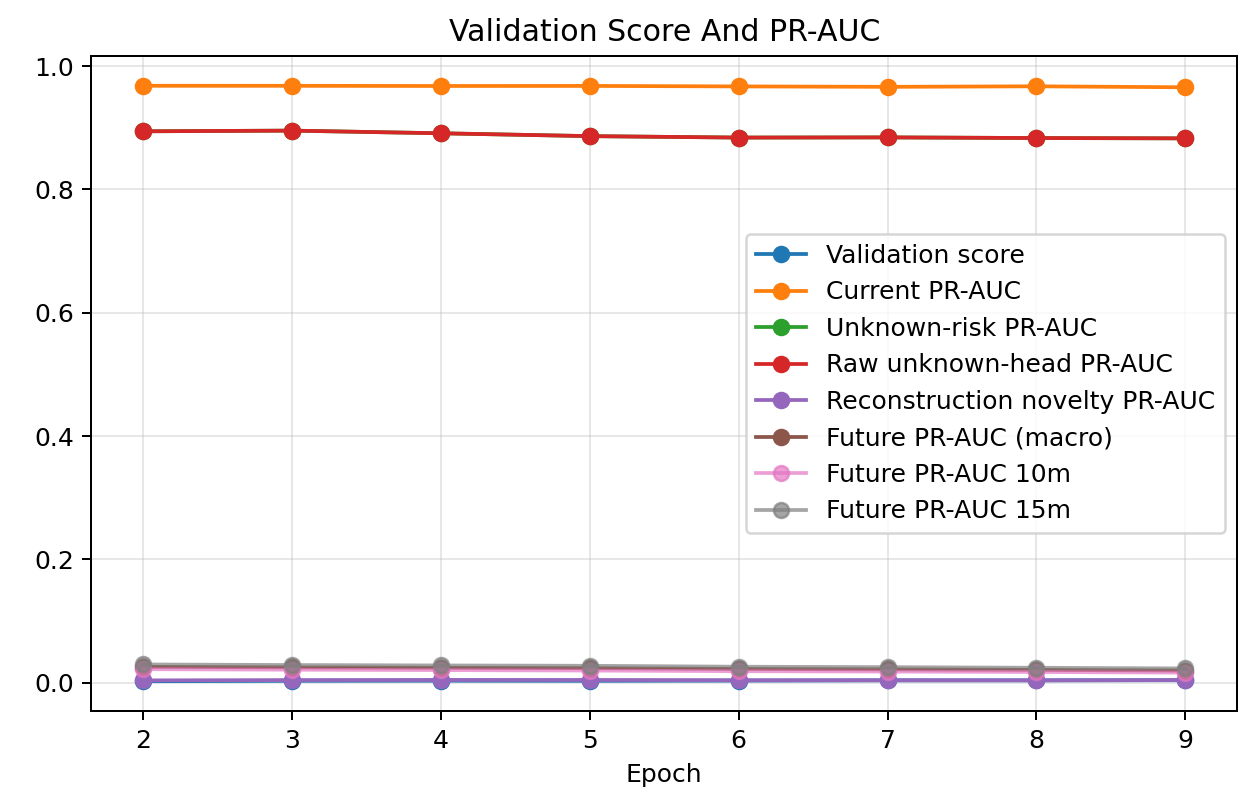
\includegraphics[width=0.9\textwidth]{v3_validation_score_pr_auc.png}
    \caption{Validation score and PR-AUC across downstream refinement epochs. The global validation score is shown together with current-detection, unknown-risk, and future-warning PR-AUC indicators used during checkpoint ranking.}
    \label{fig:contribnew_validation_score_pr_auc}
\end{figure}

\begin{figure}[H]
    \centering
    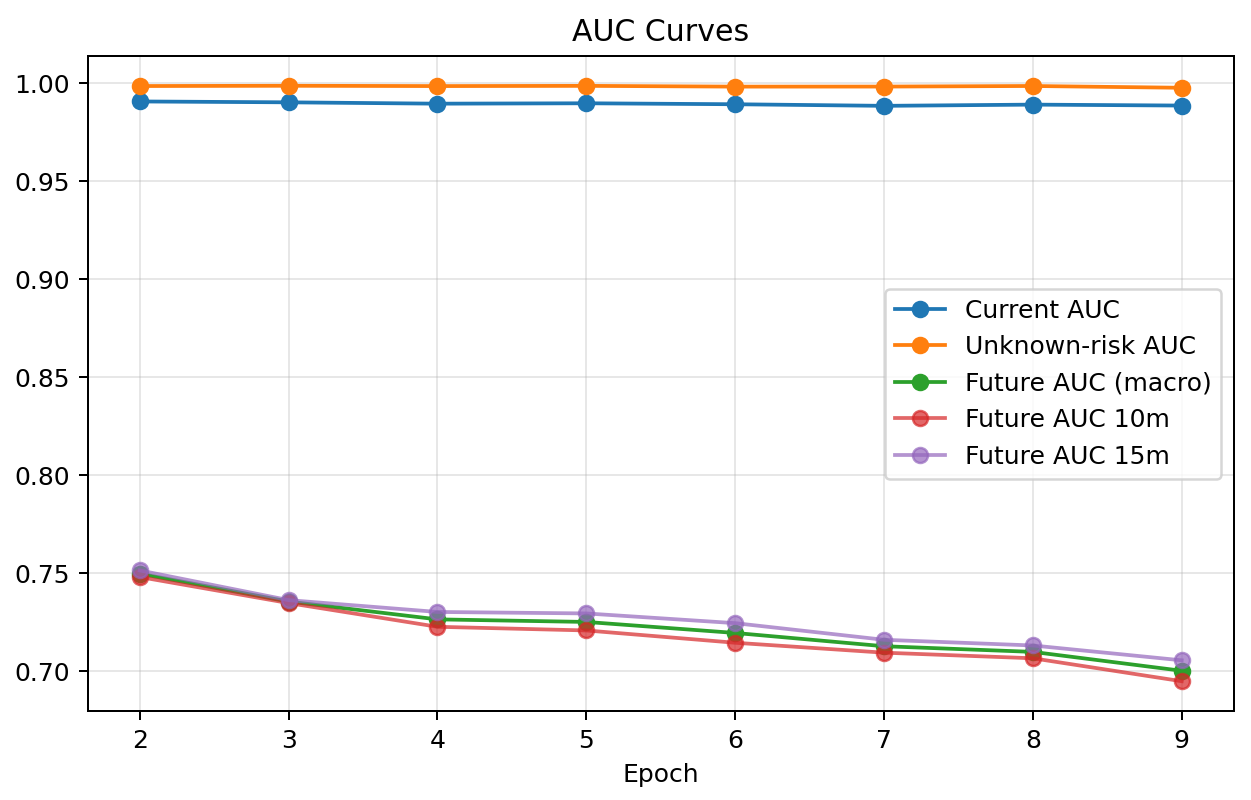
\includegraphics[width=0.9\textwidth]{v3_validation_auc_curves.png}
    \caption{Validation AUC trends across downstream refinement epochs. This view summarizes the ranking behavior of the current-detection, unknown-risk, and future-warning branches over the retained checkpoints.}
    \label{fig:contribnew_validation_auc_curves}
\end{figure}

\begin{figure}[H]
    \centering
    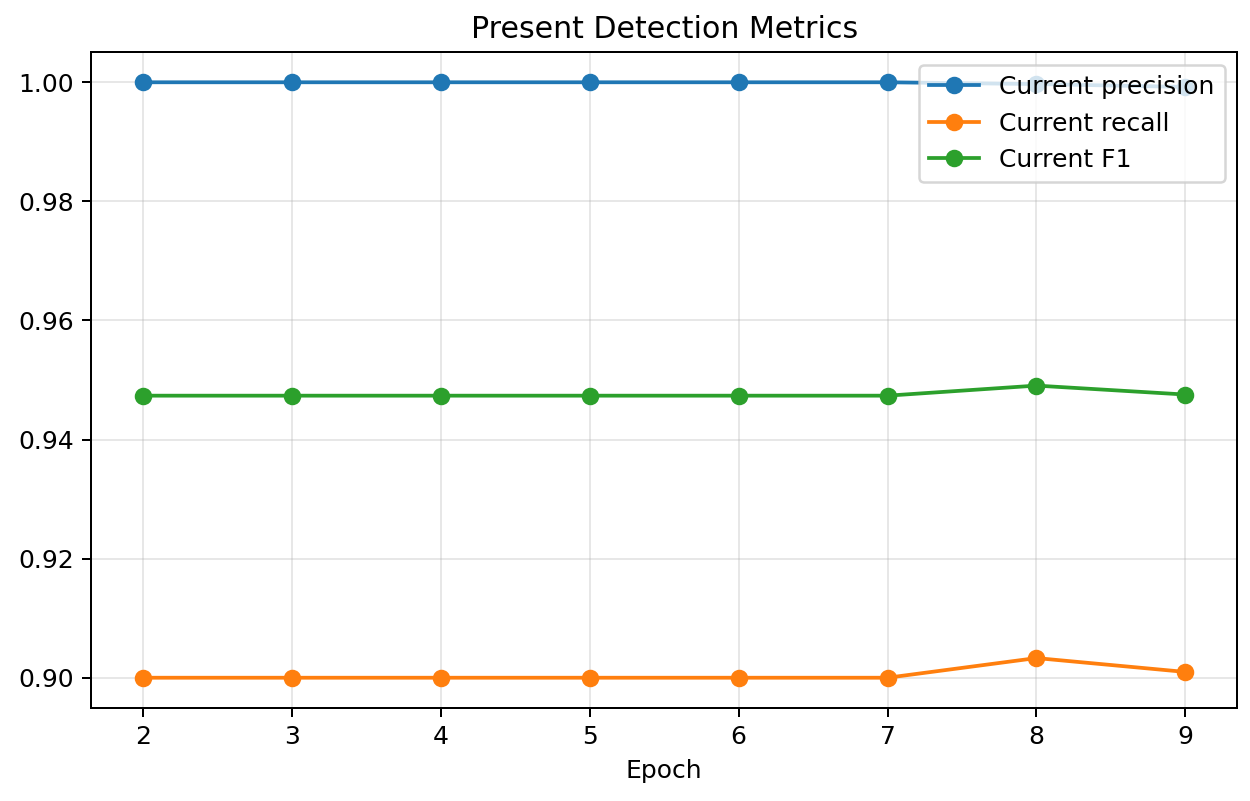
\includegraphics[width=0.9\textwidth]{v3_validation_present_detection_metrics.png}
    \caption{Present-detection validation metrics across downstream refinement epochs. Precision stays almost perfect while recall and F1 change only slightly, which confirms that the current-attack head is already saturated early.}
    \label{fig:contribnew_validation_present_metrics}
\end{figure}

\begin{figure}[H]
    \centering
    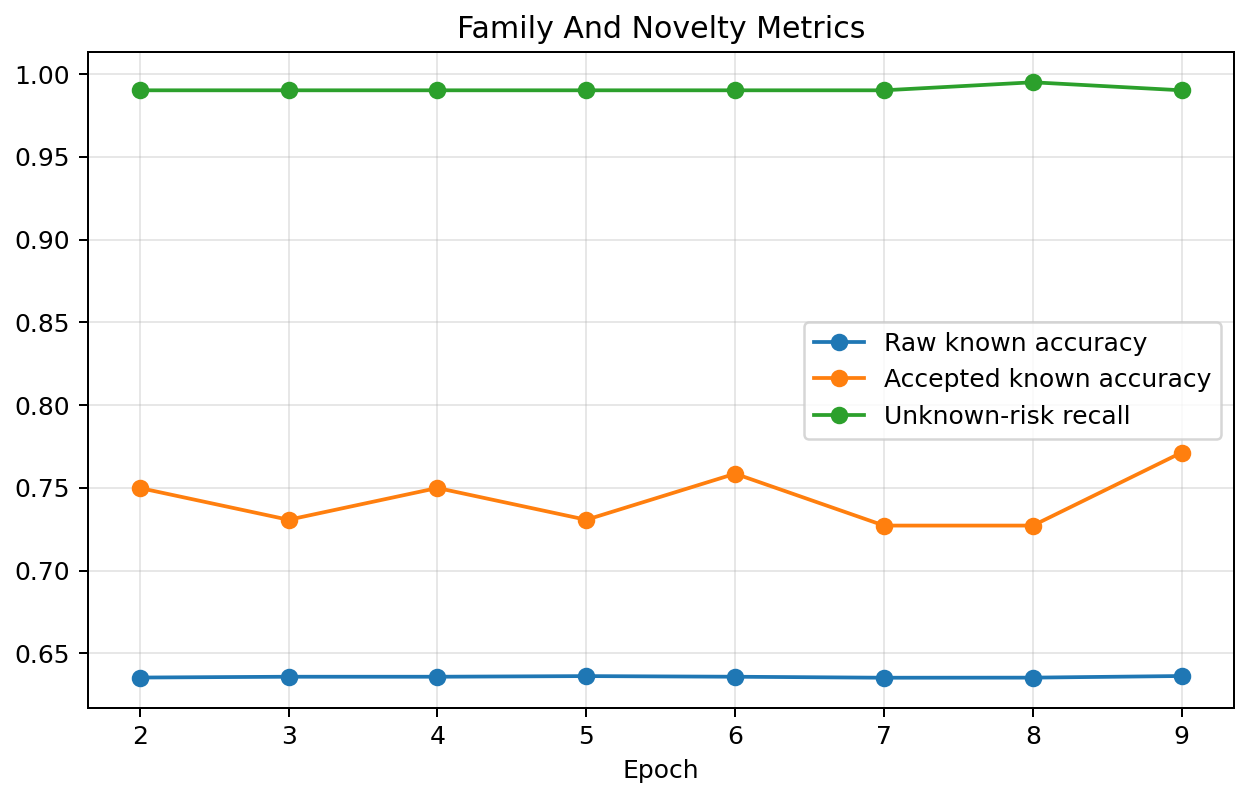
\includegraphics[width=0.9\textwidth]{v3_validation_family_novelty_metrics.png}
    \caption{Family and novelty validation metrics across downstream refinement epochs. These diagnostics show how accepted known-family accuracy and unknown-risk recall continue to influence the final checkpoint choice.}
    \label{fig:contribnew_validation_family_novelty_metrics}
\end{figure}

\subsection{Quantitative Summary Across Splits}

\begin{table}[H]
    \centering
    \small
    \caption{Summary of the downstream open-set benchmark in the revised contribution chapter. Family coverage denotes the proportion of known-attack windows for which the system accepts a family prediction at the deployed confidence threshold.}
    \label{tab:contribnew_results_summary}
    \begin{tabularx}{\textwidth}{l *{6}{>{\centering\arraybackslash}X}}
        \toprule
        Split & Current PR-AUC & Current F1 & Unknown PR-AUC & Unknown F1 & Family coverage & Raw family macro F1 \\
        \midrule
        Train & 0.979 & 0.916 & 0.961 & 0.926  & 0.058 & 0.481 \\
        Validation & 0.969 & 0.947 & 0.870 & 0.881  & 0.032 & 0.427 \\
        Test & 0.936 & 0.855 & 0.750 & 0.829  & 0.049 & 0.394 \\
        Test\_OOD & 0.969 & 0.000 & 1.000 & 0.000  & -- & -- \\
        \bottomrule
    \end{tabularx}
\end{table}

This table highlights the main pattern of the proposed contribution. The pretrained STT transfers well to the standard train, validation, and test distributions, especially for present-attack detection and standard open-set rejection. However, the strict held-out-family benchmark remains the hardest operating condition and exposes a severe threshold-transfer problem.

\subsection{Present Detection and Unknown-Risk Ranking}

Present-attack detection is the strongest task of the downstream model. The system reaches PR-AUC values of $0.979$ on train, $0.969$ on validation, and $0.936$ on test. The deployed threshold is conservative: precision remains essentially perfect on validation and test, benign false-positive rates remain close to zero, but recall decreases on the test split. This means that the learned backbone separates malicious from benign traffic well, but the selected operating point favors alert precision over maximum attack coverage.

Unknown-risk detection also performs well on the standard open-set regime. The unknown-risk PR-AUC remains high from train to validation and stays useful on test, with strong recall and low benign-and-known false-positive rates. This shows that the system can already reject a large portion of suspicious traffic instead of forcing every malicious window into the known family taxonomy.

\begin{figure}[H]
    \centering
    
\includegraphics[width=1\textwidth]{validation_current_curves.png}
    \caption{Validation curves for present-attack detection in the revised IDS. The ranking behavior remains strong on the validation distribution.}
    \label{fig:contribnew_validation_current_curves}
\end{figure}

\begin{figure}[H]
    \centering
    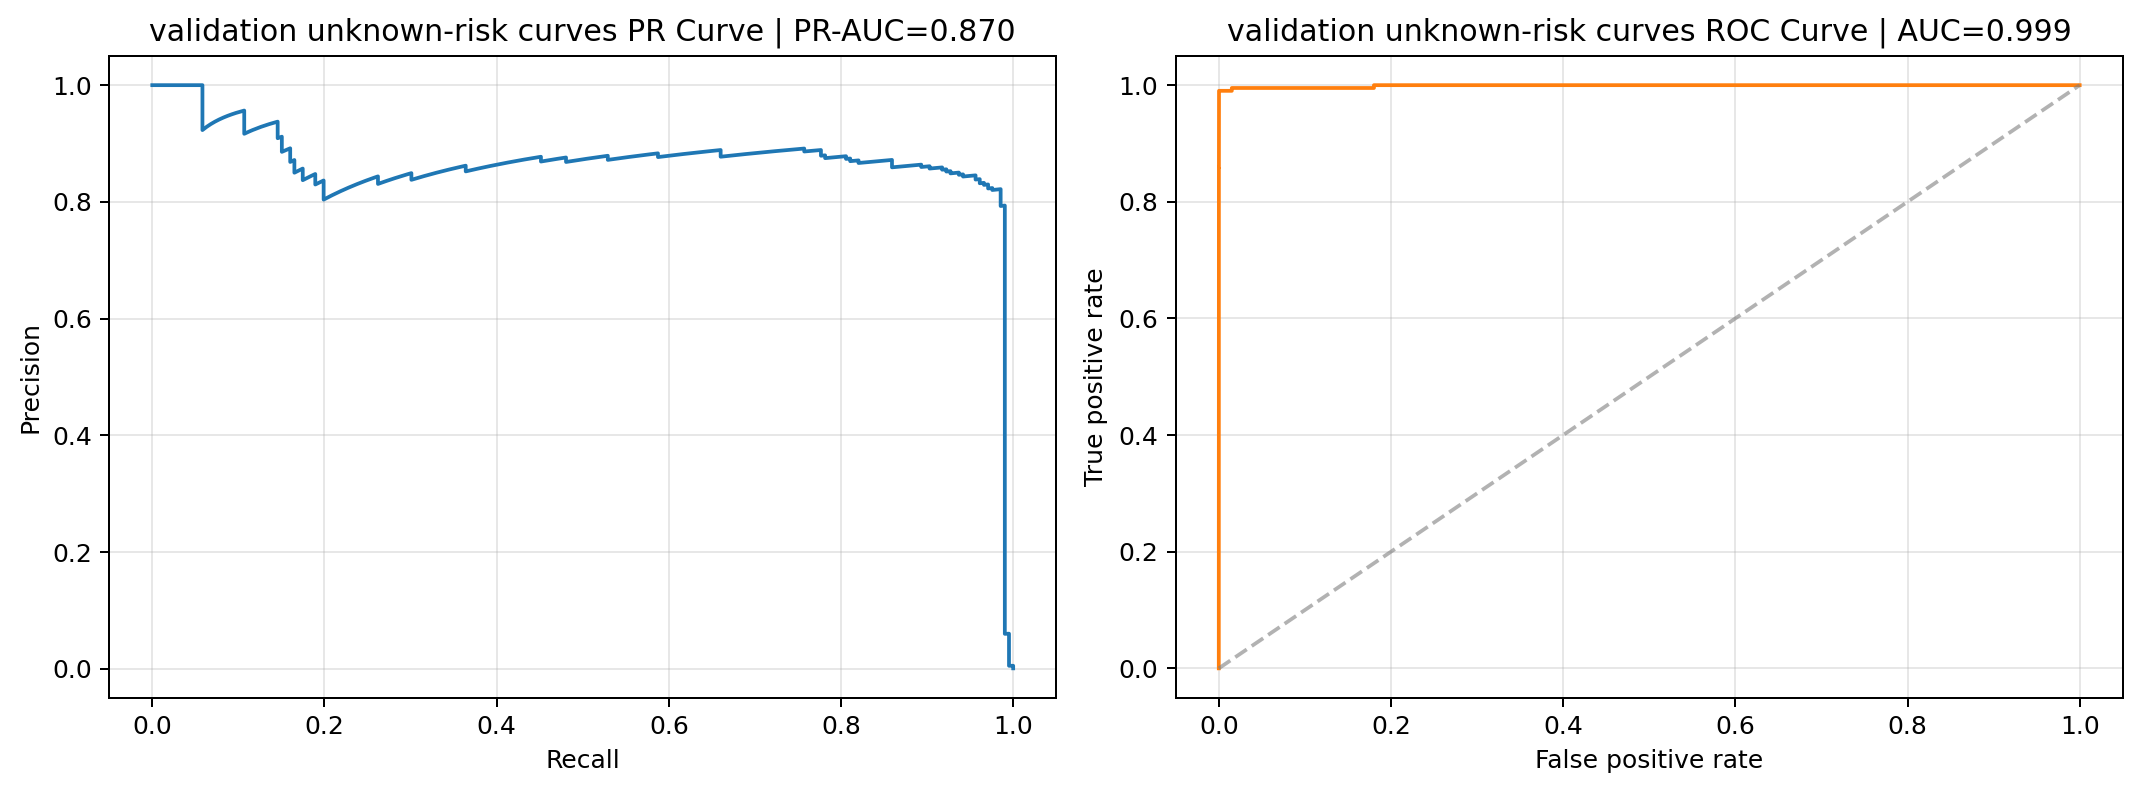
\includegraphics[width=1\textwidth]{validation_ood_curves.png}
    \caption{Validation curves for unknown-risk detection in the revised IDS. The figure confirms strong novelty-ranking behavior on the validation distribution.}
    \label{fig:contribnew_validation_ood_curves}
\end{figure}



\subsection{Held-Out-Family Failure on \texttt{test\_ood}}

The most important limitation appears on \texttt{test\_ood}. At the deployed thresholds, the current-attack head, the unknown-risk head, and the future-warning heads all collapse to zero operational recall and F1, despite very high ranking metrics such as PR-AUC. This is not a contradiction. It means that the score ordering still separates samples, but the validation-selected thresholds do not transfer to the score distribution induced by the fully held-out family.

\begin{figure}[H]
    \centering
    
\includegraphics[width=0.9\textwidth]{test_current_curves.png}
    \caption{Generalization curves on the standard test split. The current-attack head still shows strong ranking behavior under the standard evaluation regime.}
    \label{fig:contribnew_test_current_curves}
\end{figure}

\begin{figure}[H]
    \centering
    
\includegraphics[width=0.9\textwidth]{test_ood_current_threshold_sweep.png}
    \caption{Threshold-transfer failure on \texttt{test\_ood}. The validation-selected operating point lies outside the useful decision region for the held-out-family benchmark.}
    \label{fig:contribnew_test_ood_threshold_sweep}
\end{figure}

\section{Main Findings of the Revised Contribution}

The revised contribution chapter leads to four main findings. First, the STT backbone learns a useful traffic representation through masked self-supervision and transfers well to binary attack detection. Second, the unknown-risk branch already provides practical value on the standard open-set regime by preventing aggressive forced assignment into known families. Third, future warning and family attribution are informative but still less mature than present detection. Fourth, the strict held-out-family benchmark remains unresolved: the main limitation of the current system is not ranking quality alone, but the lack of threshold robustness under distribution shift. Consequently, the proposed architecture provides a strong and well-grounded hierarchical IDS foundation, but fully reliable held-out-family generalization still requires stronger OOD calibration and more robust open-set adaptation mechanisms.































% -------------------------------------------------------------------
% CHAPTER 5: CONCLUSION
% -------------------------------------------------------------------
\part{General Conclusion}

This thesis presented the \textbf{Hybrid Masked Spatio-Temporal Transformer (HM-STT)}, a novel architecture for NIDS. By treating network flows as spatio-temporal volumes and utilizing tubelet embeddings, our model learns robust representations without labor-intensive labeling. Our analysis of SAFE (2025) and Falcon (2021) highlights the industry's trajectory towards self-supervision. HM-STT contributes by offering a unified model that respects the intrinsic structure of network data. Future work will focus on optimizing final efficiency for edge deployment and integrating GNNs to model inter-flow correlations.

% -------------------------------------------------------------------
% REFERENCES
% -------------------------------------------------------------------
\printbibliography

\end{document}